\PassOptionsToPackage{unicode}{hyperref}

%Präsentationsmodus:
%\documentclass[aspectratio=1610, professionalfonts, 9pt]{beamer}

%Druckmodus:
\documentclass[aspectratio=1610, professionalfonts, 9pt]{beamer}
%\usepackage[usenames,dvipsnames]{xcolor}
\usefonttheme[onlymath]{serif}
\usetheme[showtotalframes]{tudoflw}
\setbeamertemplate{bibliography item}{\insertbiblabel}
\ifluatex
  \usepackage{polyglossia}
  \setmainlanguage{german}
\else
  \ifxetex
    \usepackage{polyglossia}
    \setmainlanguage{german}
  \else
    \usepackage[german]{babel}
  \fi
\fi
    
% Mathematik
\usepackage{amsmath}
\usepackage{amssymb}
\usepackage{animate}
\usepackage{mathtools}
\usepackage{cancel}
\usepackage{xcolor}
\definecolor{tugreen}{HTML}{84b819}
\usepackage{hyperref}
\usepackage{bookmark}
\usepackage{verbatim}
\usepackage[]{algorithm2e}
\usepackage{pgf,tikz}
\usepackage{pgfplots}
\usetikzlibrary{arrows}
\usepackage{multirow}
\usepackage{ulem}
\usepackage{caption}
\usepackage{subcaption}
\usepackage[backend=biber]{biblatex}
\bibliography{LDV-Quellen}

\SetKw{Parameters}{Parameters}

\definecolor{wqwqwq}{rgb}{0.3764705882352941,0.3764705882352941,0.3764705882352941}
\definecolor{ududff}{rgb}{0.30196078431372547,0.30196078431372547,1.}
\definecolor{ffqqqq}{rgb}{1.,0.,0.}
%\usepackage[numbers]{natbib}

\DeclareMathOperator*{\argmax}{arg\,max}
\DeclareMathOperator*{\argmin}{arg\,min}

%%%%%%%%%%%%%%%%%%%%%%%%%%%%%%%%%%%%%%%%%%%%%%%%%%%%%%%%%%%%%%%%%%%%%%%%%%%%%%%%
%%%%%							Axel Krüger	   							   %%%%%
%%%%%							TU Dortmund								   %%%%%
%%%%%					Lehrstuhl für Förder- und Lagerwesen			   %%%%%
%%%%%					Logistische Datenverarbeitung					   %%%%%
%%%%% 						Sommersemester 2019							   %%%%%
%%%%%%%%%%%%%%%%%%%%%%%%%%%%%%%%%%%%%%%%%%%%%%%%%%%%%%%%%%%%%%%%%%%%%%%%%%%%%%%%

%Titel:
\title[MPC-Planner]{MPC Planner for mobile robots in Complex Environment}
%Autor
\author[A.~Abouelkhair]{Abdulrahman Abouelkhair\\ Supervised by: Mojtaba MasoudiNejad, M.Sc.}
%Lehrstuhl/Fakultät
\institute[FLW]{\small Lehrstuhl für Förder- und Lagerwesen \\  Fakultät Maschinenbau}
%Titelgrafik 
\titlegraphic{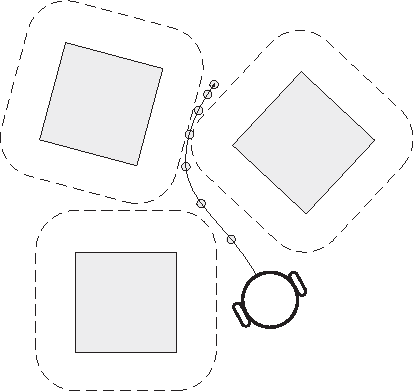
\includegraphics[width=0.3\textwidth]{pictures/mpc_robot}}
\date[SoSe 2019]{Master Thesis - Automation \& Robotics}


\AtBeginSection[]{
  \begin{frame}
  \vfill
  \centering
  \begin{beamercolorbox}[sep=8pt,center,shadow=false,rounded=true]{title in head/foot}
    \setlength{\fboxrule}{1pt}
    \fcolorbox{tugreen}{white}{\usebeamerfont{title}\insertsectionhead\par}
  \end{beamercolorbox}
  \vfill
  \end{frame}
}

 %Damit das Inhaltsverzeichnis nummeriert ist
\setbeamertemplate{sections/subsections in toc}[sections numbered]
\setbeamertemplate{subsection in toc}[subsections numbered]


\begin{document}

\maketitle

\begin{frame}
    \frametitle{Agenda}
    %\tableofcontents[pausesections]
    \tableofcontents
\end{frame}

% Organisatorisches
\section*{Organisatorisches}

	\begin{frame}
		\frametitle{Kontakt}
		\begin{tabular}{ll}
			Anschrift & Technische Universität Dortmund\\
			& Lehrstuhl für Förder- und Lagerwesen (FLW)\\
			& LogistikCampus\\
			& Joseph-von-Fraunhofer-Str. 2-4 \\
			& 44227 Dortmund\\[0.1cm]
			Name & Mojtaba MasoudiNejad, M.Sc.\\[0.1cm]
			Raum& A4.06\\[0.1cm]
			Telefon& +49 231 755-3236\\[0.1cm]
			Mail& mojtaba.masoudinejad@tu-dortmund.de\\[0.1cm]
			Sprechstunde& flexibel nach Vereinbarung\\[0.1cm]
		\end{tabular}
	\end{frame}

	\begin{frame}
		\frametitle{Master Präsentation Termine}
		\begin{tabular}{ll}
		Ort & FLW / A3.16\\[0.1cm]
		Zeit & 18 Oct. 2019 um 11:00 - 11:25 \\[0.1cm]
		Examiners &  Moritz Roidl, Dipl.-Inform.\\
		&Mojtaba MasoudiNejad, M.Sc.
		\end{tabular}\\[1cm]
	\end{frame}

	\begin{frame}
	\frametitle{Literatur}
	    \begin{columns}[T]
	        \begin{column}{0.49\textwidth}
	            \begin{itemize}%[<+->] Kommentar entfernen falls jeder Punkt einzeln erscheinen soll
					\item Title: Springer Handbook of Robotics
					\item Author: Khatib, Oussama ; Siciliano, Bruno
					\item Link: \href{https://www.ub.tu-dortmund.de/katalog/titel/HT019024543}{https://www.ub.tu-dortmund.de/katalog/titel/HT019024543}
	        	\end{itemize}
	        \end{column}
	        \begin{column}{0.49\textwidth}
	        	\centering
	            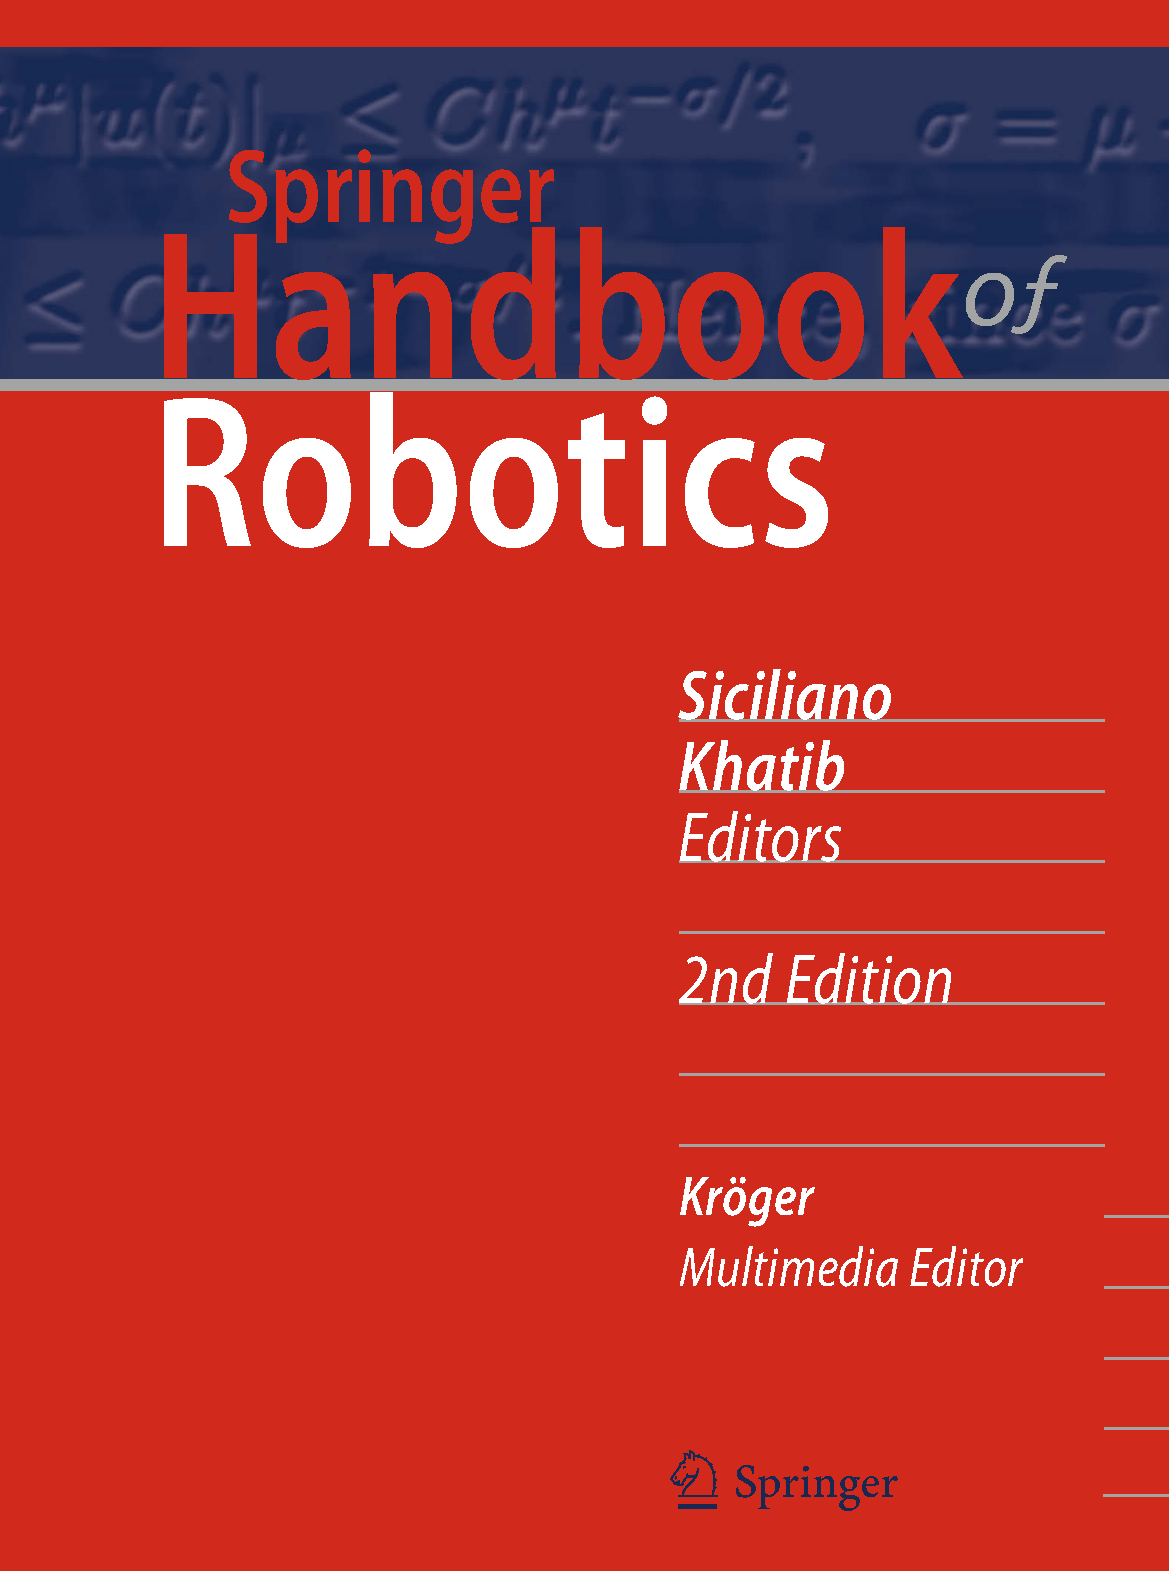
\includegraphics[scale=0.25]{pictures/springer_robotics.pdf}
	        \end{column}
	    \end{columns}
	\end{frame}

	\begin{frame}
		\frametitle{Literatur}
		\begin{columns}[T]
			\begin{column}{0.49\textwidth}
				\begin{itemize}%[<+->] Kommentar entfernen falls jeder Punkt einzeln erscheinen soll
					\item Title: Model Predictive Control : Theory, Computation, and Design 
					\item Author: Diehl, Moritz ; Mayne, David Q ; Rawlings, James Blake
					\item Link: \href{https://www.ub.tu-dortmund.de/katalog/titel/HT019602243}{https://www.ub.tu-dortmund.de/katalog/titel/HT019602243}
				\end{itemize}
			\end{column}
			\begin{column}{0.49\textwidth}
				\centering
				\includegraphics[scale=0.305]{pictures/mpc_book_cover.png}
			\end{column}
		\end{columns}
	\end{frame}

	\begin{frame}
		\frametitle{Literatur}
		\begin{columns}[T]
			\begin{column}{0.49\textwidth}
				\begin{itemize}%[<+->] Kommentar entfernen falls jeder Punkt einzeln erscheinen soll
					\item Title: Numerical Optimization
					\item Author: Nocedal, Jorge ; Wright, Stephen J
					\item Link: \href{https://www.ub.tu-dortmund.de/katalog/titel/HT014641035}{https://www.ub.tu-dortmund.de/katalog/titel/HT014641035}
				\end{itemize}
			\end{column}
			\begin{column}{0.49\textwidth}
				\centering
				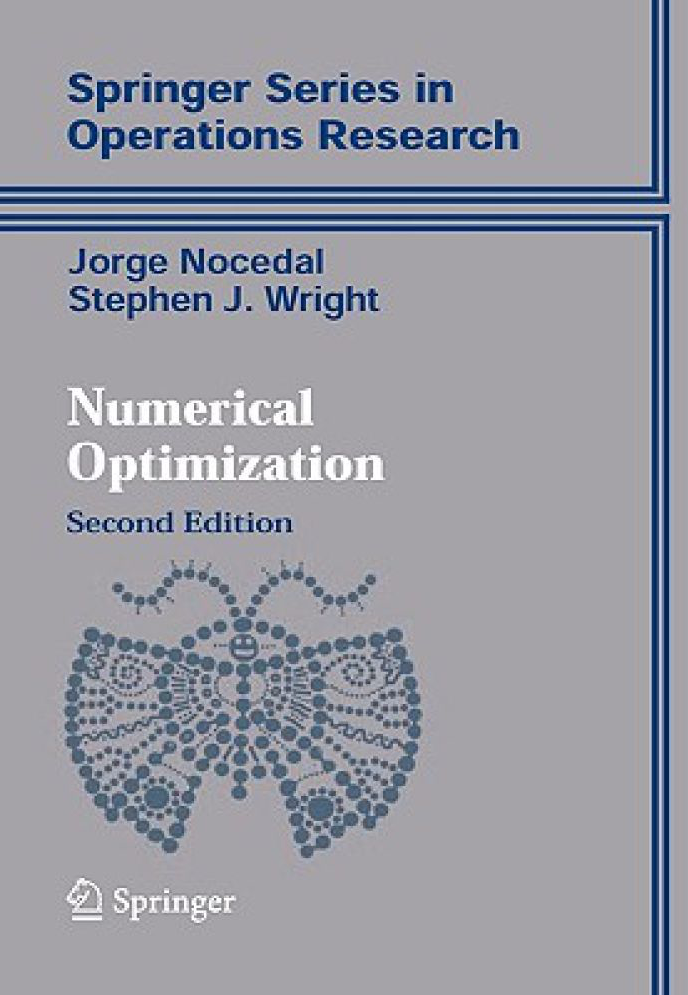
\includegraphics[scale=0.2]{pictures/numerical_optimization.png}
			\end{column}
		\end{columns}
	\end{frame}

% Ziele
\section*{Ziele}
\begin{frame}
\frametitle{Lernziele}
Am Ende des Semesters können Sie
\begin{itemize}
\item die Grundbegriffe der Statistik unterscheiden und erläutern,
\pause
\item grundlegende statistische und wahrscheinlichkeitstheoretische Kennzahlen bestimmen und interpretieren,
\pause
\item ausgewählte maschinelle Lernverfahren in ihren Grundzügen erklären und einsetzen,
\pause
\item Aufgabentypen des maschinellen Lernens unterscheiden und für den jeweiligen Aufgabentyp geeignete Verfahren benennen,
\pause
\item erlernte Modelle validieren und testen,
\pause
\item Ergebnisse der Datenanalyse visualisieren,
\pause
\item die Anforderungen an ein Datenbanksystem benennen und erläutern.
\end{itemize}
\end{frame}
%\begin{frame}
%\frametitle{Der rote Faden}
%% Für Bilder Argument T benutzen:
%    \begin{columns}[T]
%        \begin{column}{0.49\textwidth}
%            \begin{itemize}%[<+->] Kommentar entfernen falls jeder Punkt einzeln erscheinen soll
%            	\item[$\,\blacktriangleright$] Daten aufnehmen
%            	\begin{itemize}
%            		\item Was sind Daten?
%            		\item Woher kommen Daten?
%            	\end{itemize}	
%            	\item[$\,\blacktriangleright$] Daten speichern
%            		\begin{itemize}
%            			\item Welche Anforderungen gibt es an Datenbanken?
%            			\item Wie kann ich Daten in einer relationalen Datenbank abrufen?
%            		\end{itemize}
%            	\item[$\,\blacktriangleright$] Daten auswerten
%            	\begin{itemize}
%            		\item Welche Möglichkeiten zur Auswertung gibt es?
%            		\item Was ist maschinelles Lernen und was sind die Einsatzmöglichkeiten?
%            		\item Wie prüfe ich ein erlerntes Modell?
%            		\item Wie kann ich Ergebnisse visualisieren?
%            	\end{itemize}
%        	\end{itemize}
%        \end{column}
%        \begin{column}{0.49\textwidth}
%            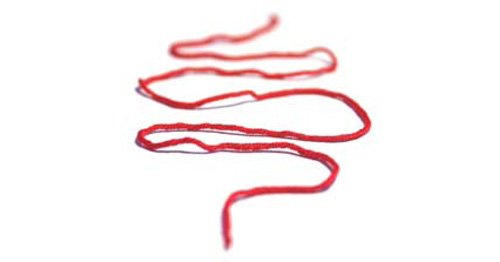
\includegraphics[width=\textwidth]{images/roter-faden.jpg}
%        \end{column}
%    \end{columns}
%\end{frame}

% Einführung
\section{Introduction and Motivation}

	\begin{frame}
		\frametitle{Introduction}
		\begin{columns}
			\begin{column}{0.49\textwidth}
				\begin{itemize}
					\item \onslide<1->{Novel Strategy} \\[0.7cm]
					\item \onslide<2->{Decentralized Navigation} \\[0.7cm]
					\item \onslide<3->{Optimal Motion Planning} \\[0.7cm]
					\item \onslide<5->{Autonomous Decision Making}
				\end{itemize}
			\end{column}
			\pause
			\begin{column}{0.49\textwidth}
				\centering
				\onslide<4->{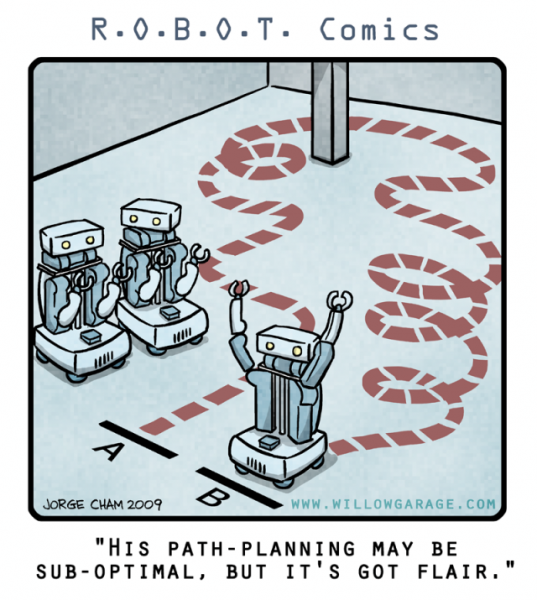
\includegraphics[width=0.85\textwidth]{pictures/robot_comic.png}}
			\end{column}
		\end{columns}
	\end{frame}
	
	\begin{frame}
		\frametitle{Latest Approaches and Motivation}
	    \begin{columns}[T]
	        \begin{column}{0.49\textwidth}
	            \begin{itemize}%[<+->] Kommentar entfernen falls jeder Punkt einzeln erscheinen soll
					\item \onslide<1->{Environment Previous Knowledge}\\[0.5cm]
					\item \onslide<3->{Maximum speed $\leq 1.5 m/s$} \\[1cm]
					\item \onslide<4->{This approach has the potential to improve : \\[0.5cm]
					\begin{itemize}
						\item system performance \\[0.2cm]
						\item fast path towards goal
					\end{itemize}
					}
	        	\end{itemize}
	        \end{column}
	        \begin{column}{0.49\textwidth}
	        	\begin{itemize}%[<+->] Kommentar entfernen falls jeder Punkt einzeln erscheinen soll
	        		\item \onslide<2->{Global Planner}
	        	\end{itemize}
        		\centering
        		\only<1>{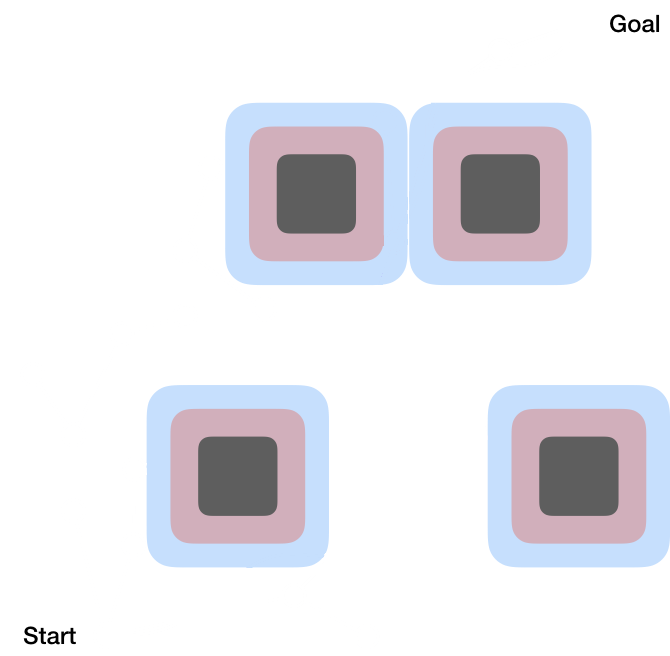
\includegraphics[width=0.8\textwidth]{pictures/figure_1.png}}
        		\only<2>{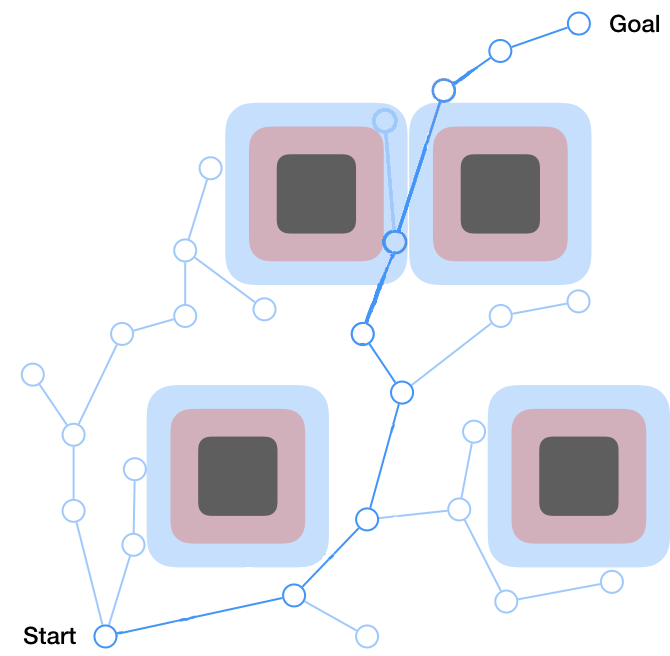
\includegraphics[width=0.8\textwidth]{pictures/figure_2.png}}
        		\only<3->{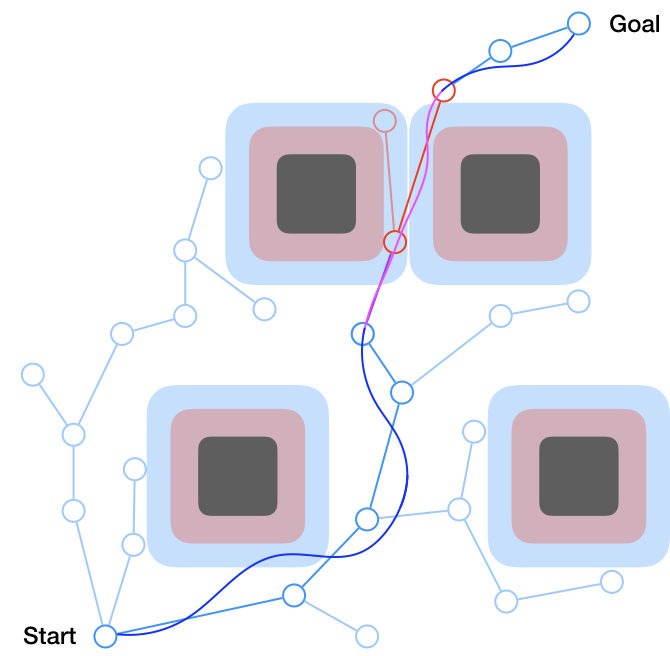
\includegraphics[width=0.8\textwidth]{pictures/figure.png}}
	        \end{column}
	    \end{columns}
	\end{frame}
	
	\begin{frame}
		\begin{block}{Proposed Approach\footnotemark}
			\begin{itemize}
				\pause
				\item On-line trajectory planning \\ [0.4cm]
				\pause
				\item Without \textit{global planner} \\ [0.4cm]
				\pause
				\item Without \textit{map} \\ [0.4cm]
				\pause
				\item Dynamic Environment, e.g. \textit{(pedestrian, multi-robots)} \\ [0.4cm]
				\pause
				\item Robot speed $> 1.5 m/s$ \\ [0.4cm]
				\pause
				\item Smooth navigation \\ [0.4cm]
				\pause
				\item Deadlock free
			\end{itemize}
		\end{block}
		\footnotetext[1]{
			Hoy, Michael and Matveev, Alexey S. and Savkin, Andrey V. 
			\say{
				\href{https://www.cambridge.org/core/journals/robotica/article/algorithms-for-collisionfree-navigation-of-mobile-robots-in-complex-cluttered-environments-a-survey/ADA8F6F7E30123629A26B08DA0C79C8C}{
					\textcolor{tudark}{Algorithms for collision-free navigation of mobile robots in complex cluttered environments: a survey}
				}
			}. In Cambridge University Press (2016).
		}
	\end{frame}

	\begin{frame}
		\begin{columns}[T]
			\begin{column}{0.49\textwidth}
			\begin{itemize}%[<+->] Kommentar entfernen falls jeder Punkt einzeln erscheinen soll
				\item Current Approach: \\[0.2cm]
				\begin{itemize}
					\item Laser Scanner + Map \\[0.1cm]
					\item Robot's estimated location 
				\end{itemize}
			\end{itemize}
			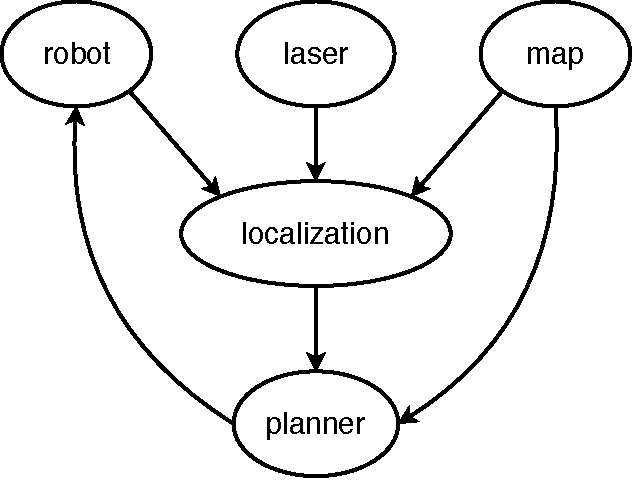
\includegraphics[scale=0.67]{pictures/navigation_ros_2.pdf}
			\end{column}
			\pause
			\begin{column}{0.49\textwidth}
				\begin{itemize}%[<+->] Kommentar entfernen falls jeder Punkt einzeln erscheinen soll
					\item Proposed Approach: \\[0.2cm]
					\begin{itemize}
						\item Robot localization \\[0.1cm]
						\item Obstacles location 
					\end{itemize}
				\end{itemize}
				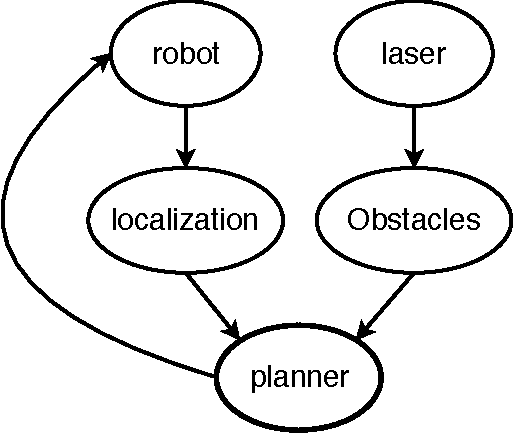
\includegraphics[scale=0.75]{pictures/navigation_ros_3.pdf}
			\end{column}
		\end{columns}
	\end{frame}

	\begin{frame}
		\frametitle{Model Predictive Control}
		\centering
		\only<1>{\animategraphics[loop,controls,width=0.75\textwidth]{2}{pictures/mpc_group/MPC_scheme_basic-}{0}{6}}
		\only<2>{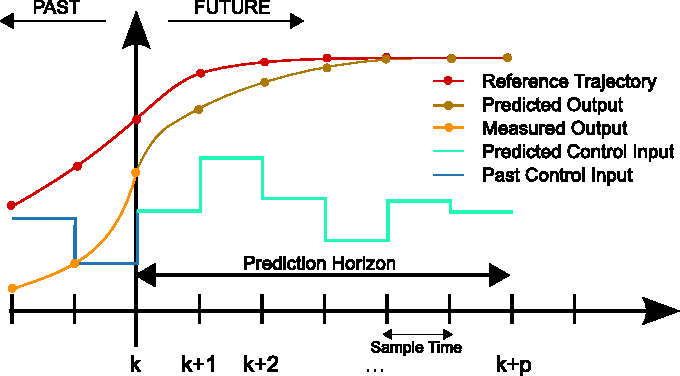
\includegraphics[scale=1.0]{pictures/mpc_group/MPC_scheme_basic-7.pdf}}
	\end{frame}

	\begin{frame}
		\frametitle{On-line Trajectory (prediction horizon)}
		\centering
		\movie[width=0.42\textwidth, height=0.45\textwidth]
		{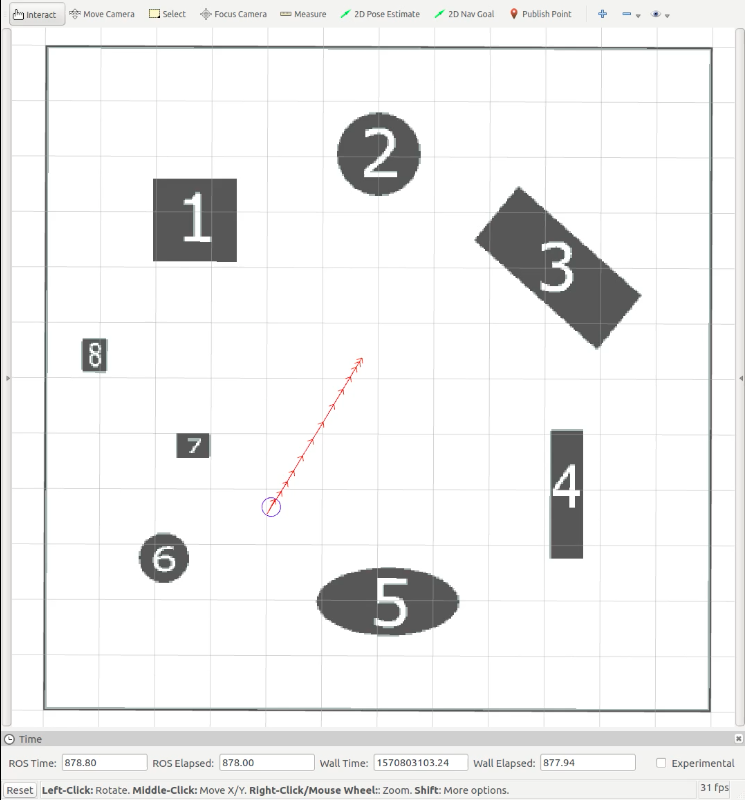
\includegraphics[width=0.42\textwidth]{pictures/path.png}}{videos/path.mov}
	\end{frame}

	\begin{frame}
		\frametitle{NMPC Optimization Problem Schematic}
		\centering
		\only<1>{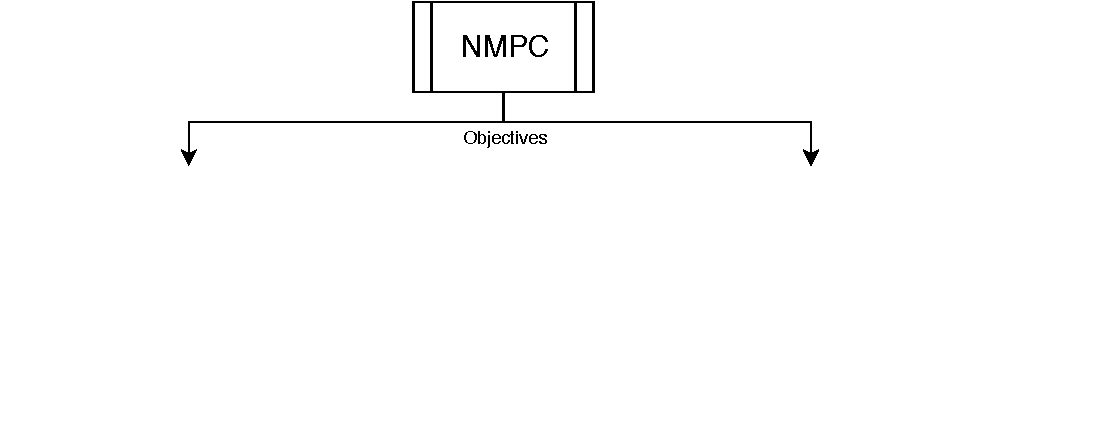
\includegraphics[scale=0.8]{pictures/mpc_planner_group/mpc_planner_0.pdf}}
		\centering
		\only<2>{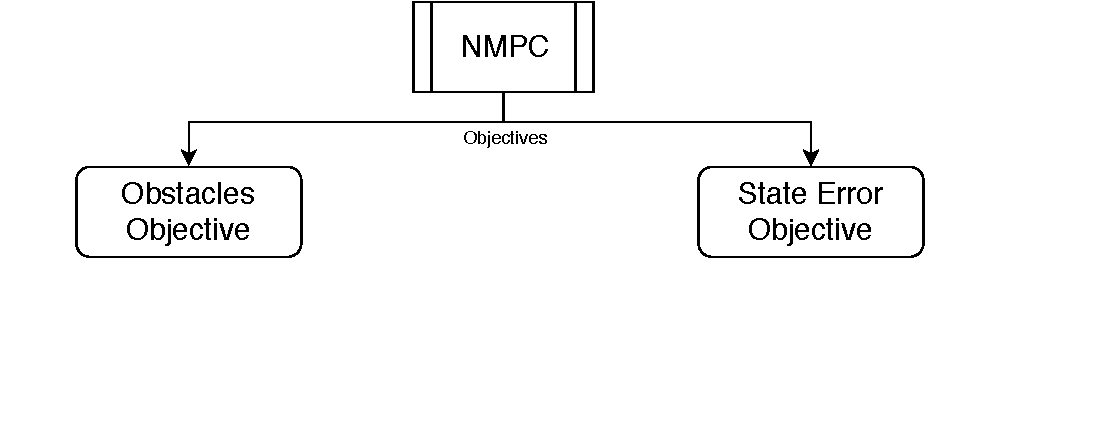
\includegraphics[scale=0.8]{pictures/mpc_planner_group/mpc_planner_1.pdf}}
		\centering
		\only<3>{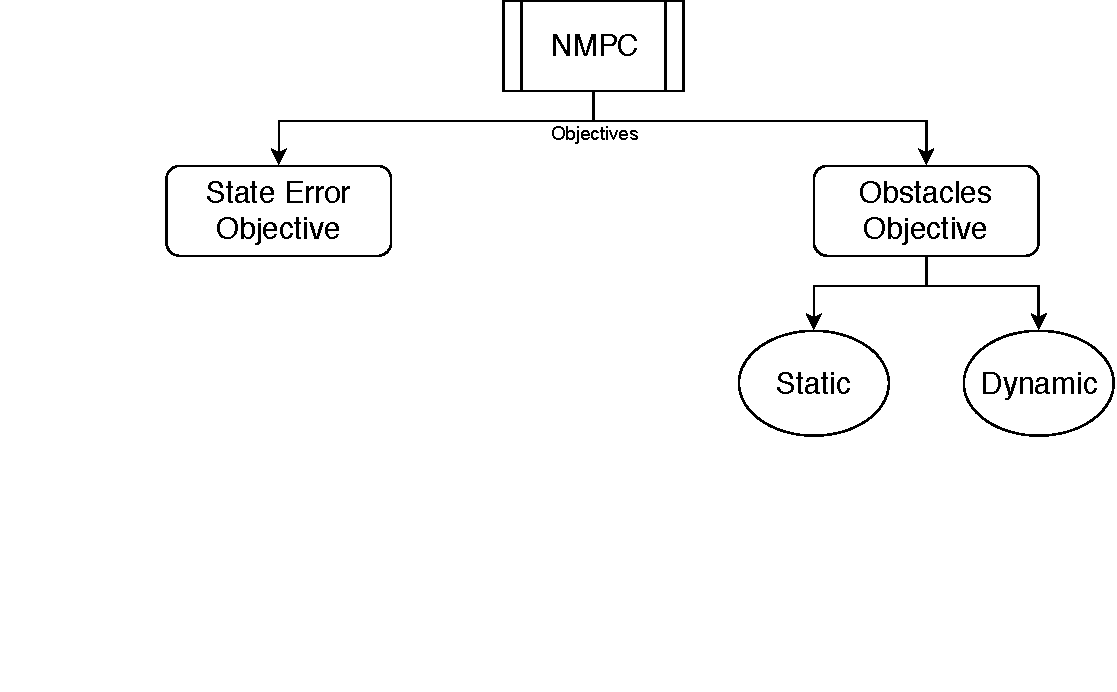
\includegraphics[scale=0.8]{pictures/mpc_planner_group/mpc_planner_2.pdf}}
		\centering
		\only<4>{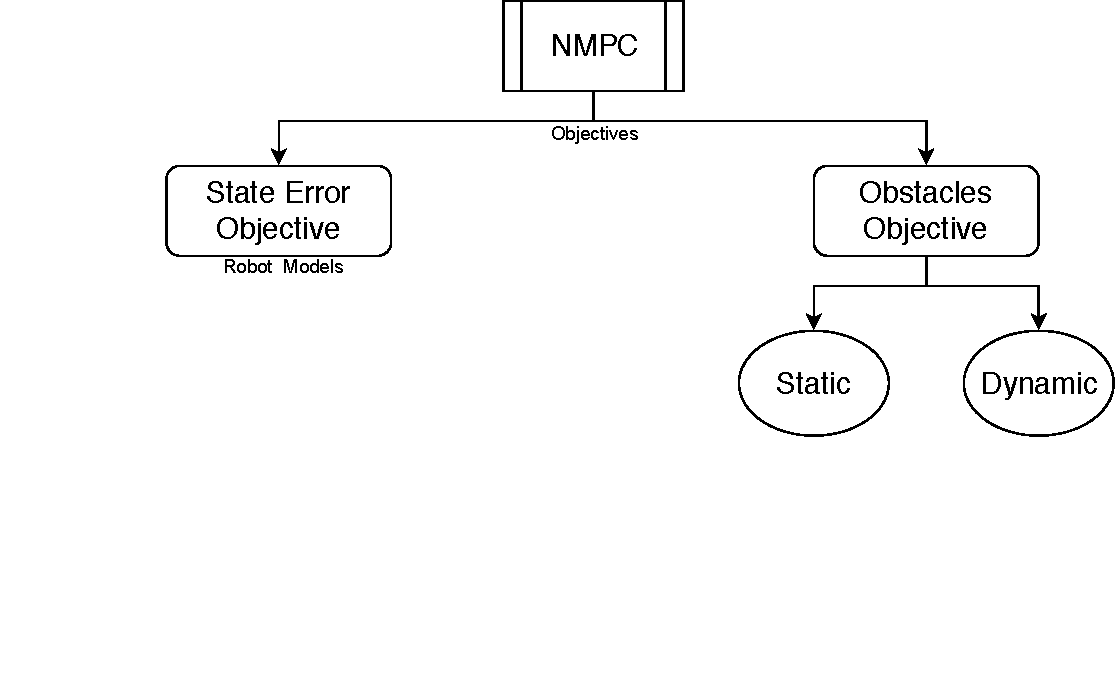
\includegraphics[scale=0.8]{pictures/mpc_planner_group/mpc_planner_3.pdf}}
		\centering
		\only<5>{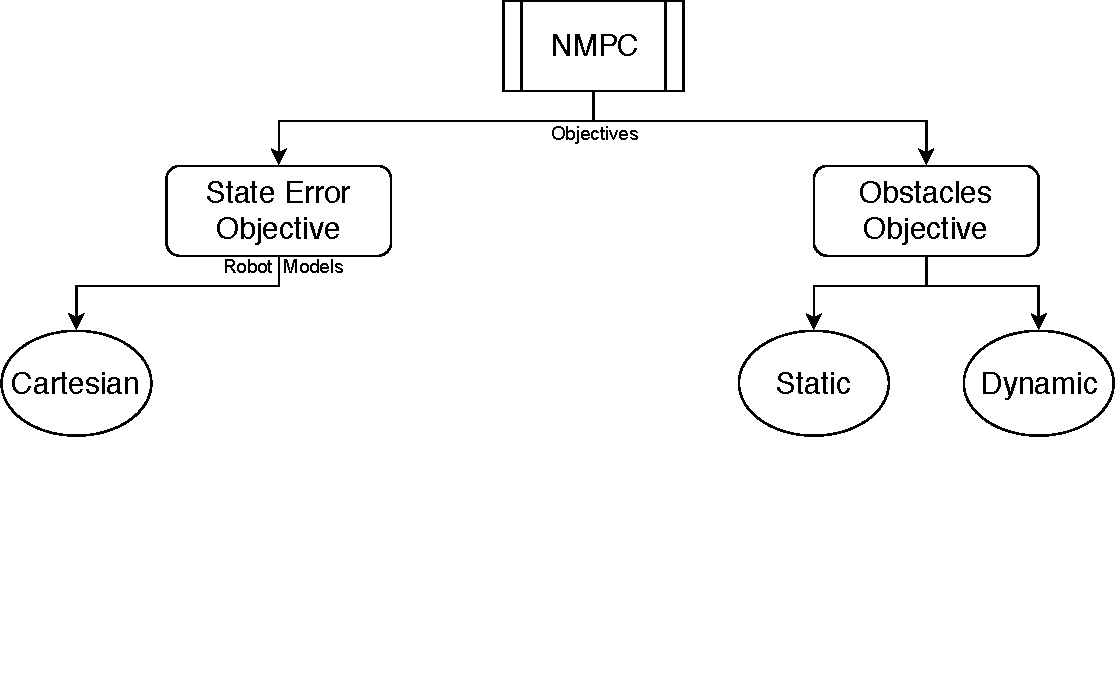
\includegraphics[scale=0.8]{pictures/mpc_planner_group/mpc_planner_4.pdf}}
		\centering
		\only<6>{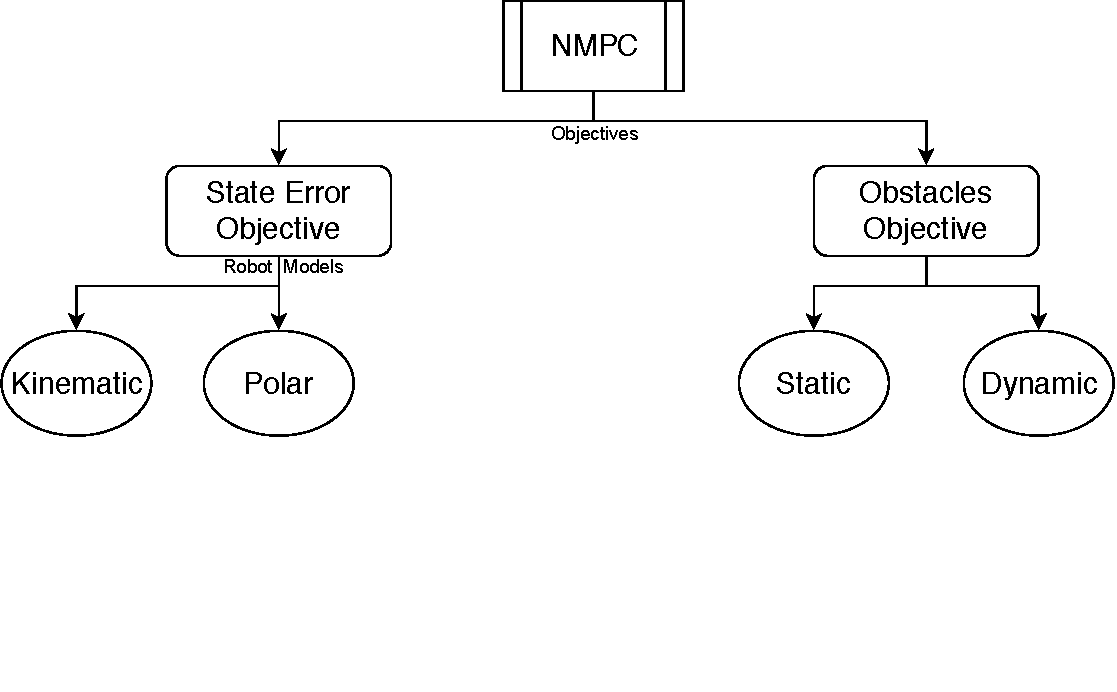
\includegraphics[scale=0.8]{pictures/mpc_planner_group/mpc_planner_5.pdf}}
		\centering
		\only<7>{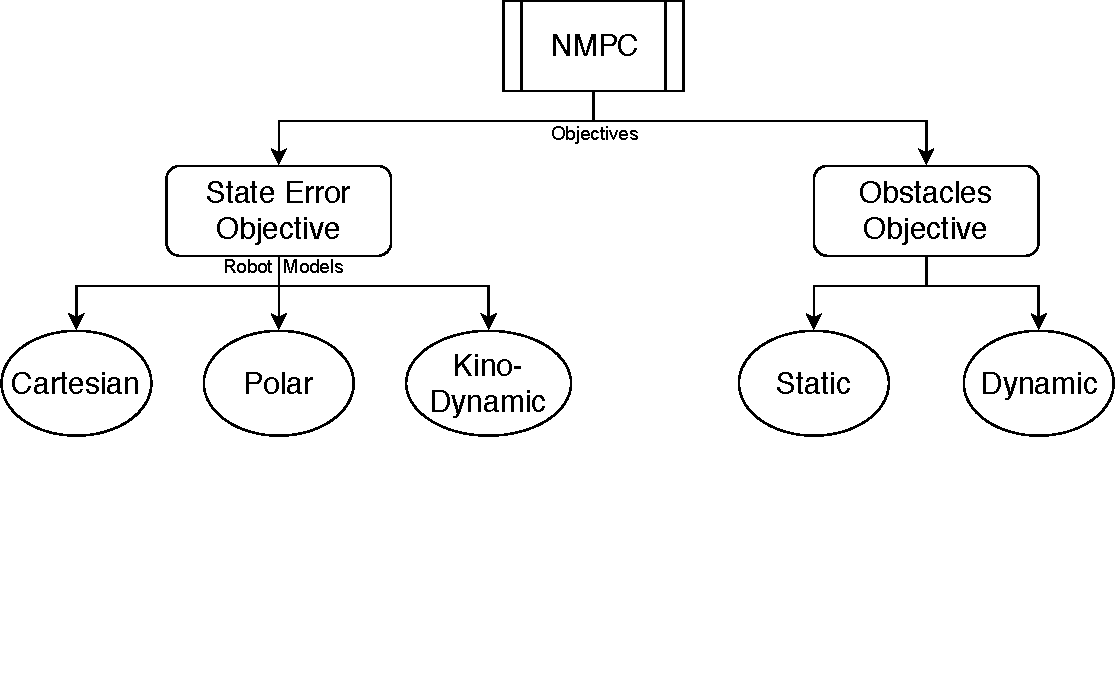
\includegraphics[scale=0.8]{pictures/mpc_planner_group/mpc_planner_6.pdf}}
	\end{frame}

% Statistik
\section{Obstacles Formulation}

	\begin{frame}
		\frametitle{Robot Environment}
		\begin{columns}[T]
			\begin{column}{0.3\textwidth}
				\begin{itemize}
					\item Static obstacles location \\[1.0cm]
					\item Dynamic obstacles trajectory
				\end{itemize}
			\end{column}
			\begin{column}{0.7\textwidth}
				\centering
				\animategraphics[loop,controls,width=0.7\linewidth]{2}{pictures/robot_env_group/robot_env-}{0}{8}
				%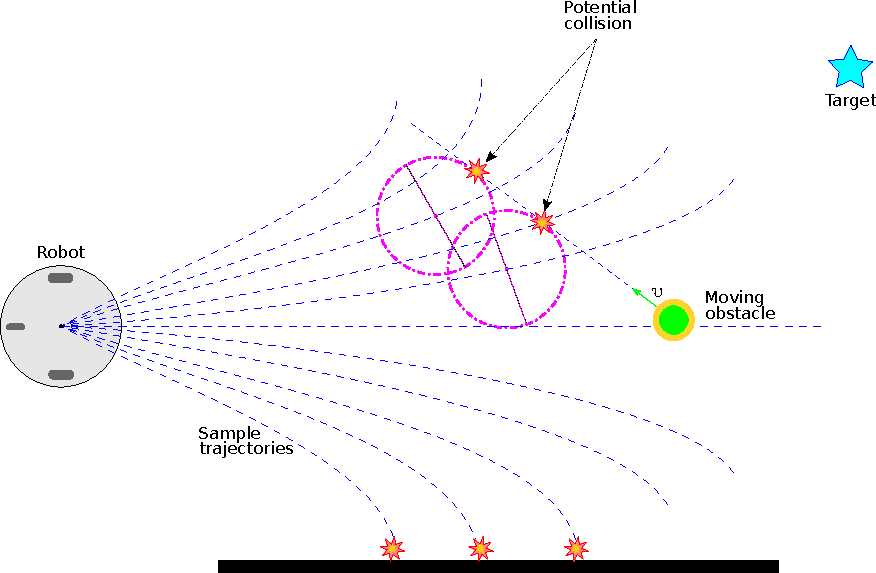
\includegraphics[scale=0.7]{pictures/robot_env.pdf}
			\end{column}
		\end{columns}
	\end{frame}

	\begin{frame}
		\frametitle{Laser Scanner}
		\begin{columns}[T]
			\begin{column}{0.42\textwidth}
				\centering
				\onslide<1->{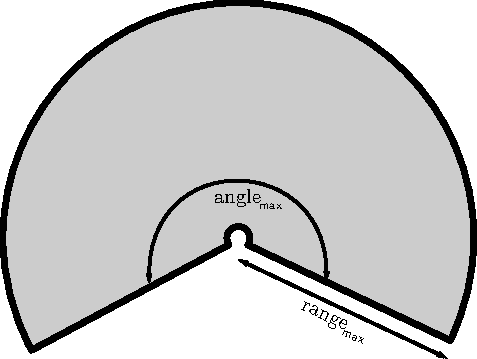
\includegraphics[scale=0.45]{pictures/laser_ranges.pdf}}
				\onslide<2->{
				\begin{block}{Laser scanner message}
					\[\overrightarrow{data}(k) = \left\{
					\begin{array}{lr}
					angle_{min} \\
					angle_{max} \\
					\overrightarrow{angle}_{inc}, \quad \qquad \forall \enspace \delta \in \overrightarrow{angle}_{inc} \\
					range_{min} \\
					range_{max} \\
					\overrightarrow{ranges}, \qquad \qquad \forall \enspace \sigma \in \overrightarrow{ranges}
					\end{array}
					\right.
					\]
				\end{block}
				}
			\end{column}
			\begin{column}{0.52\textwidth}
				\centering
				 \onslide<3->{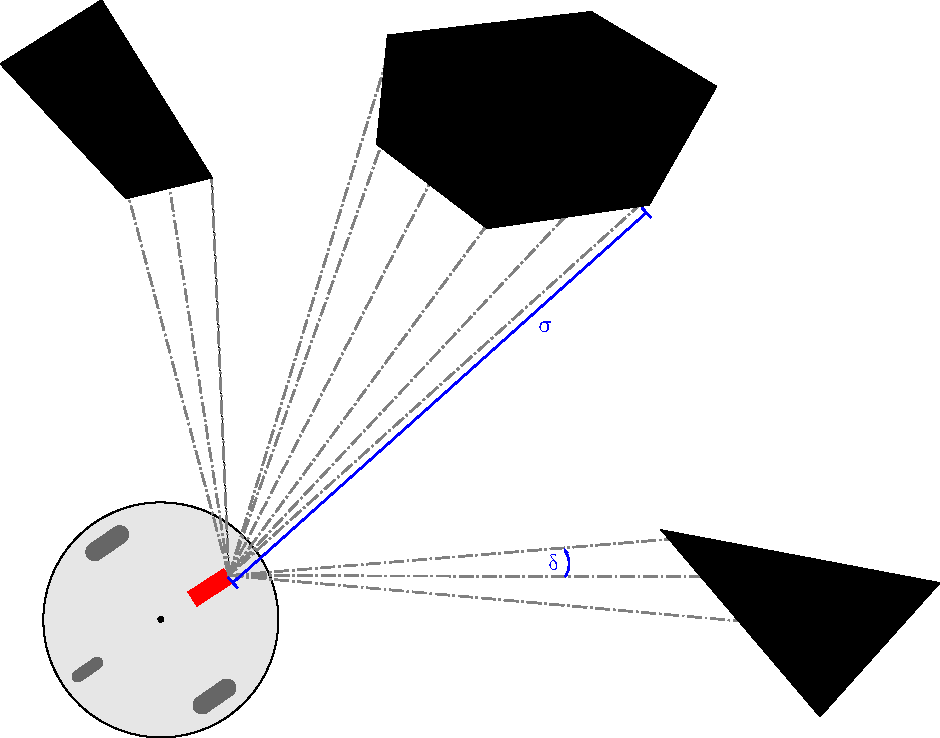
\includegraphics[scale=0.51]{pictures/robot_laser.pdf}}
			\end{column}
		\end{columns}
	\end{frame}

	\begin{frame}
		\frametitle{Homogeneous Transformation}
		\begin{columns}[T]
			\begin{column}{0.4\textwidth}
				\onslide<2->{
				\begin{block}{Rotation Matrix regarding $Z$-axis}
					\[
						T_z = 
						\begin{pmatrix}
							\cos\theta_z & -\sin\theta_z & 0 & x_{trns} \\
							\sin\theta_z &  \cos\theta_z & 0 & y_{trns}  \\
							0		   & 0 			 & 1 & y_{trns}  \\
							0		   & 0			 & 0 & 1 \\
						\end{pmatrix}
					\]
				\end{block}
				}
				\onslide<3->{
				\begin{block}{Co-ordinate Transformation}
					\[
						T_{obst\_map} = 
						T_{ft\_map} T_{r\_ft} T_{lsr\_r}
						\begin{pmatrix}
							x_{obst} \\
							y_{obst} \\
							z_{obst} \\
							1 
						\end{pmatrix}
					\]
				\end{block}
				}
			\end{column}
			\begin{column}{0.55\textwidth}
				\centering
				\onslide<1->{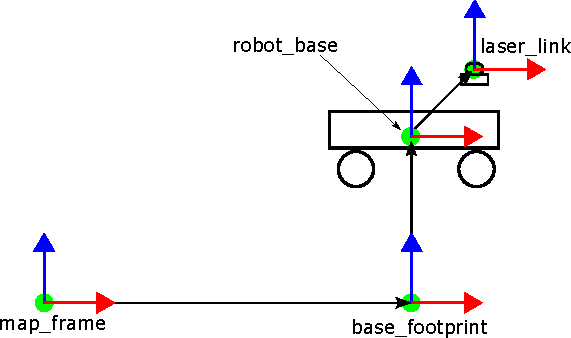
\includegraphics[scale=0.9]{pictures/laser_robot_frame.pdf}}
			\end{column}
		\end{columns}
	\end{frame}

	\begin{frame}
		\frametitle{Homogeneous Transformation}
		\begin{columns}[T]
			\begin{column}{0.49\textwidth}
				\begin{itemize}
					\item $
					T_{footprint\_map} \enspace \text{ }=
					\begin{pmatrix}
						\cos\theta_r & -\sin\theta_r & 0 & x_{r} \\
						\sin\theta_r & \cos\theta_r & 0 & y_{r} \\
						0 & 0 & 1 & 0 \\
						0 & 0 & 0 & 1 \\
					\end{pmatrix}
					$
					\item $
					T_{robot\_footprint} \enspace= 
					\begin{pmatrix}
						1 & 0 & 0 & 0 \\
						0 & 1 & 0 & 0 \\
						0 & 0 & 1 & -0.125 \\
						0 & 0 & 0 & 1 \\
					\end{pmatrix}
					$
					\item $
					T_{laser\_robot} \qquad= 
					\begin{pmatrix}
						1 & 0 & 0 & 0 \\
						0 & 1 & 0 & -0.245 \\
						0 & 0 & 1 & -0.051 \\
						0 & 0 & 0 & 1 \\
					\end{pmatrix}
					$
				\end{itemize}
			\end{column}
			\begin{column}{0.49\textwidth}
				\centering
				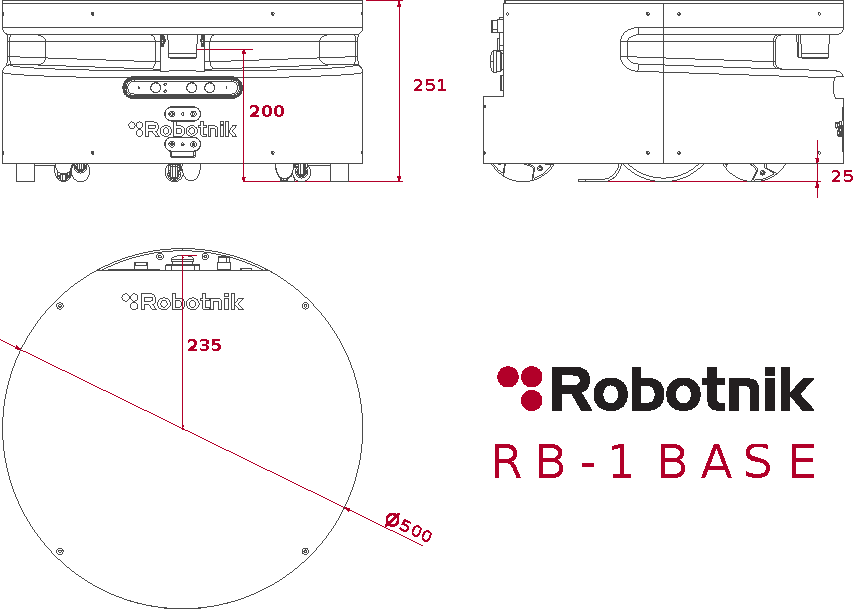
\includegraphics[scale=0.5]{pictures/robotnik.pdf}
			\end{column}
		\end{columns}
	\end{frame}

	\begin{frame}
		\frametitle{Saved Obstacles Frame}
		\centering
		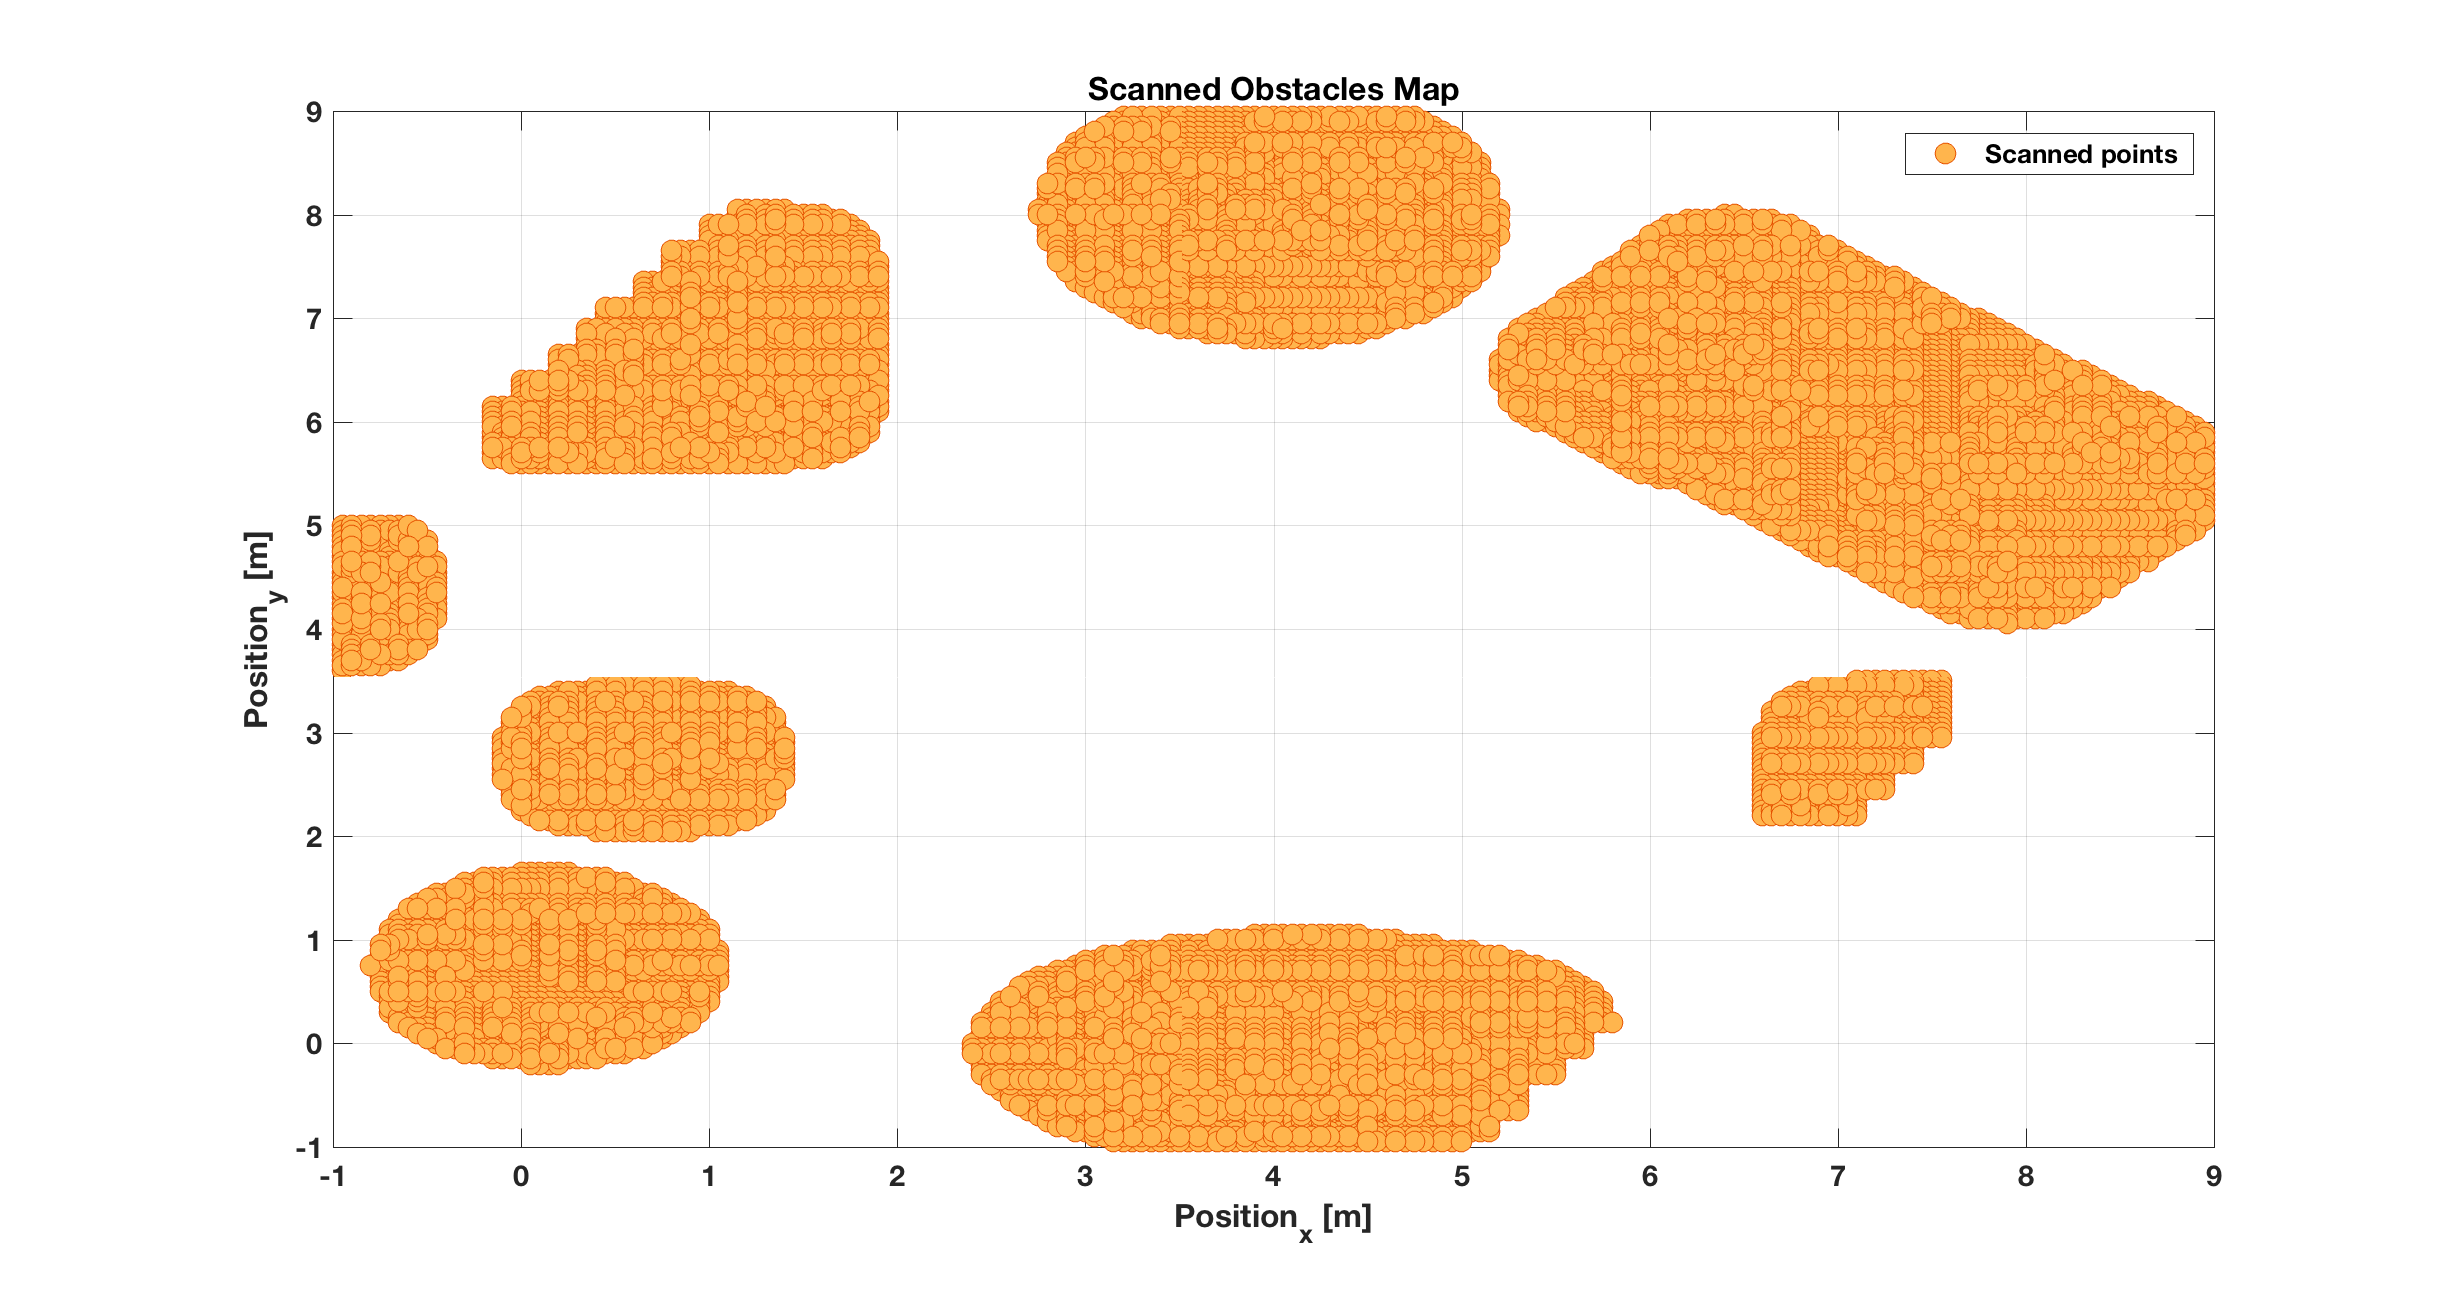
\includegraphics[scale=0.46]{pictures/intial_map.eps}
	\end{frame}

	\begin{frame}
		\frametitle{Cluster + Fitting Algorithm}
		\onslide<1->{
		\begin{block}{Density-Based Spatial Clustering of Applications with Noise (DBSCAN)}
			Statistical search algorithm
		\end{block}
		\begin{block}{Least Square Fitting Ellipse (LSFE)}
			Numerical fitting algorithm for each set of data.
		\end{block}
		}
		\begin{columns}[T]
			\onslide<2->{
			\begin{column}{0.32\textwidth}
				\begin{itemize}
					\item Edged data points
				\end{itemize}
				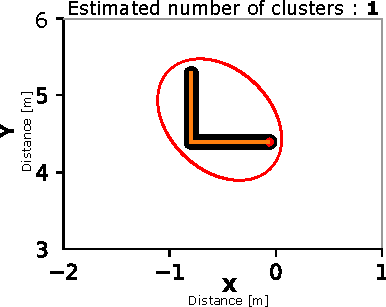
\includegraphics[scale=0.65]{pictures/lsellipse1.pdf}
			\end{column}
			}
			\onslide<3->{
			\begin{column}{0.32\textwidth}
				\begin{itemize}
					\item Concave data points
				\end{itemize}
				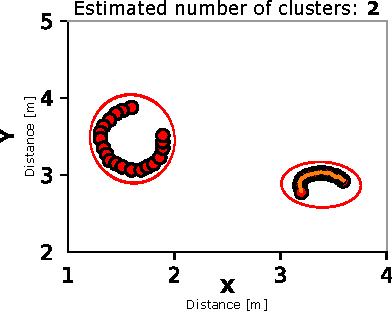
\includegraphics[scale=0.65]{pictures/lsellipse2.pdf}
			\end{column}
			}
			\onslide<4->{
			\begin{column}{0.32\textwidth}
				\begin{itemize}
					\item Lined-curved data points
				\end{itemize}
				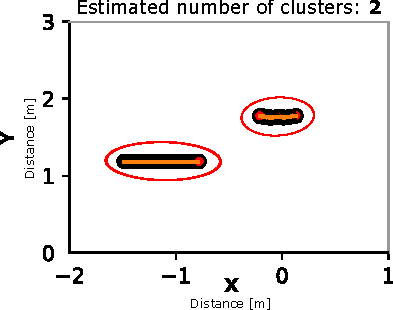
\includegraphics[scale=0.65]{pictures/lsellipse3.pdf}
			\end{column}
			}
		\end{columns}
	\end{frame}

	\begin{frame}
		\frametitle{Fitted Frame}
		\centering
		\includegraphics[scale=0.13]{pictures/map_clustered.eps}
	\end{frame}

	\begin{frame}
		\frametitle{Dynamic Obstacles Tracking}
		\begin{columns}[T]
			\begin{column}{0.4\textwidth}
				\onslide<2->{
				\begin{block}{Dyn. obstacles estimation}
					\begin{align*}
						&\hat{\mathbf{x}}_{i,k} = 
						\begin{pmatrix}
							\hat{x}_{i,k} \\
							\hat{y}_{i,k} \\
							\hat{\theta}_{i,k}
						\end{pmatrix},
						\qquad \qquad \hat{\mathbf{x}}_{i,k} =
						\begin{pmatrix}
							\hat{v}_{i,k} \\
							\hat{\omega}_{i,k}
						\end{pmatrix}
						\\
						&\hat{\mathbf{X}}_{i,k} := \{ \hat{\mathbf{x}}_{i,k}, \hat{\mathbf{x}}_{i,k+1}, \cdots, \hat{\mathbf{x}}_{i,k+N_p} \} \\
						&\bar{\mathbf{X}}_{i,k} := \{ \bar{\mathbf{x}}_{i,k}, \bar{\mathbf{x}}_{i,k+1}, \cdots, \bar{\mathbf{x}}_{i,k+N_p}\}
					\end{align*}
				\end{block}
				}
				\onslide<3->{
				\begin{block}{Dynamic obstacles vector}
					\[
					\hat{\mathbf{Z}}_{i,k} = 
					\begin{cases}
						\hat{\mathbf{X}}_{i,k}, & \text{if } i \in I_{un} \\
						\bar{\mathbf{X}}_{i,k}, & \text{if } i \in I_{robots}.
					\end{cases}
					\]
				\end{block}
				}
			\end{column}
			\begin{column}{0.56\textwidth}
				\centering
				\onslide<1->{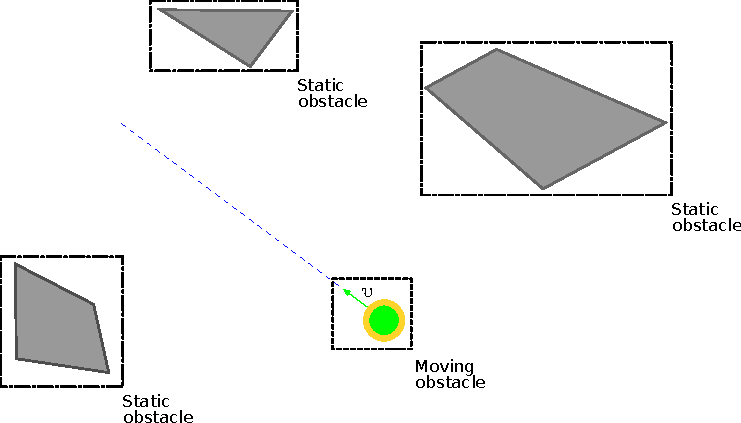
\includegraphics[scale=0.7]{pictures/robot_env_diff.pdf}}
			\end{column}
		\end{columns}
	\end{frame}

	\begin{frame}
		\frametitle{Obstacles Detection Block Diagram}
		\centering
		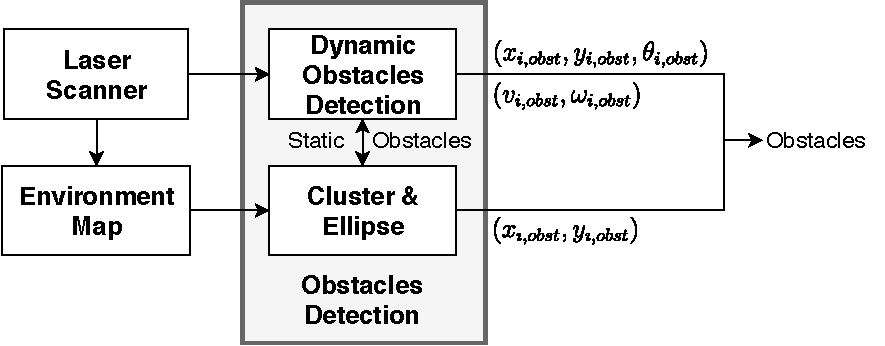
\includegraphics[scale=0.9]{pictures/block_diagram_obst_1.pdf}
	\end{frame}



% Julia
\section{Einführung in die Programmiersprache julia}
\begin{frame}
\frametitle{Überblick}
% Für Bilder Argument T benutzen:
    \begin{columns}[T]
        \begin{column}{0.65\textwidth}
            \begin{itemize}[<+->]
\item julia ist eine höhere Programmiersprache, die seit 2009 entwickelt wird
\item Hauptaugenmerk liegt auf dem numerischen und wissenschaftlichen Rechnen
\item Einfache Syntax
\item Hohe Ausführungsgeschwindigkeit
\item Einbindung von Python und R ist möglich
\item open source (MIT-Lizenz)
\item Download und Dokumentation: https://julialang.org/
\end{itemize}

        \end{column}
        \begin{column}{0.32\textwidth}
            
\includegraphics[width=\textwidth]{images/logo-julia.png}
        \end{column}
    \end{columns}
    
\end{frame}
\begin{frame}[fragile]
\frametitle{Installation von julia}
\begin{itemize}
\item Unter https://julialang.org/downloads/ die passende Datei herunterladen und installieren
\pause
\item Nach der Installation kann julia über die REPL (read-evaluate-print-loop) verwendet werden
\pause
\item Die REPL ist für das Einüben und Ausprobieren gut geeignet
\pause
\item Für größere Projekte sollte jedoch eine IDE (wie etwa Juno) oder das Jupyter Notebook verwendet werden
\pause
\item Über die REPL die folgenden Befehle ausführen um Jupyter Notebook zu installieren\footnote{Siehe https://github.com/JuliaLang/IJulia.jl}
\begin{verbatim}
julia> using Pkg
julia> Pkg.add("IJulia")
\end{verbatim}
\end{itemize}
\end{frame}
\begin{frame}
\frametitle{Problemklassen und Einzelprobleme}
\begin{block}{Problemklasse}
Eine \textit{Problemklasse} ist eine Sammlung gleichartiger Probleme, wobei diese nicht konkret formuliert sind, sondern in ihrer gemeinsamen, allgemeinen Form dargestellt sind. In der Regel kann eine Klasse über eine Funktion $f:I \rightarrow O$ repräsentiert werden, mit $I$ als Menge der Eingabe- und $O$ als Menge der Ausgabewerte.
\end{block}
Beispiele:\pause
\begin{itemize}
\item Finden eines kürzesten Weges zwischen zwei Orten\pause
\item Ermittlung möglichst ähnlicher Kundengruppen eines Unternehmens\pause
\item Erkennung von Objekten in digitalen Bilddateien\pause
\item Zuordnung von Aufgaben zu Bearbeitern\pause
\item Ermittlung der optimalen Auslagerstrategie für ein Lager
\end{itemize}
\end{frame}
\begin{frame}
\begin{block}{Einzelproblem}
Ein \textit{Einzelproblem} ist eine konkrete Instanz einer Problemklasse, d.h. es wurden alle freie Parameter der Problemklasse gewählt.
\end{block}
Beispiele:\pause
\begin{itemize}
\item Finden des kürzesten Weges zwischen der Mensa und dem HG I (bezüglich der euklidischen Norm)\pause
\item Ermittlung der ähnlichen Käufergruppen des Onlineshops www.irgendeinshop.de (bezüglich eines konkreten Ähnlichkeitsmaß)\pause
\item Unterscheidung von korrekt und nicht-korrekt verpackten Paketen auf einer Förderstrecke mittels einer festinstallierten Kamera\pause
\item Zuordnung der Mitarbeiter Meier, Müller und Schmidt auf die drei anstehenden Liefertouren X,Y und Z\pause
\item Ermittlung der Auslagerstrategie für das Lager der XYZ GmbH in Dortmund\pause
\end{itemize}
\end{frame}
\begin{frame}
\frametitle{Algorithmus}
\begin{block}{Algorithmus}
Ein \textit{Algorithmus} ist eine detaillierte und explizite Vorschrift zur schrittweisen Lösung eines Einzelproblems (einer definierten Problemklasse) durch eine Abfolge bekannter Befehle/Operationen.
\end{block}
Beispiele:\pause
\begin{itemize}
\item Dijkstra-Algorithmus (Ermittlung eines kürzesten Pfades zwischen einem Start- und Endknoten in einem Graphen)\pause
\item Euklidischer Algorithmus (Berechnung des ggT zweier natürlicher Zahlen)\pause
\item Quicksort (Algorithmus zur Sortierung von Werten einer Liste)
\end{itemize}
\end{frame}
\begin{frame}[fragile]
\frametitle{Wichtige Funktionen}
\begin{itemize}[<+->]
\item Über den Befehl \verb+?+ wird der Hilfemodus aufgerufen, über \verb+]?+ die Package-Hilfe
\item In den normalen Modus wechseln (etwa aus dem Hilfemodus heraus): [Backspace] oder eine leere Linie
\item Alle Stellen sehen wo \verb+func+ definiert ist: \verb+apropos("func")+
\item Ausführung abbrechen: [STRG] + [C]
\item Bildschirm leeren: [STRG]+[L]
\item Julia Programm ausführen: \verb+include("filname.jl")+
\item Beenden: \verb+exit()+ oder [STRG]+[D]
\end{itemize}
\end{frame}
\begin{frame}[fragile]
\begin{itemize}[<+->] 
\item Einzeilige Kommentare werden über \verb+#+ begonnen
\item Mehrzeilige Kommentare werden mit \verb+#=+ und mit \verb+=#+ beendet
\item Beispiel:
\begin{verbatim}
julia> # Ein Kommentar
julia> #= Dieser Kommentar
julia> geht über drei Zeilen. Durch "?" gelangt man in den
julia> Hilfemodus wo etwa "pi" gesucht werden kann =#
help?> pi
\end{verbatim}
\item Die Ausgabe kann über \verb+;+ unterdrückt werden
\item Der letzte Wert wird in der Variable \verb+ans+ gespeichert
\begin{verbatim}
julia> 2+2*2
6
julia> ans
6
\end{verbatim}
\end{itemize}
\end{frame}
\begin{frame}[fragile]
\frametitle{Variablen}
\begin{itemize}[<+->] 
\item Eine Variable in julia ist ein Name mit einem assoziierten Wert
\item In vielen Programmiersprachen, wie etwa Java, muss der Datentyp einer Variable bei der Deklaration explizit angegeben werden, z.B.:\\
\begin{verbatim}
java> int x = 5;
\end{verbatim}
\item In julia wird eine Typenangabe nicht benötigt:
\begin{verbatim}
julia> x = 5;                       # Die Zuweisung erfolgt über =
\end{verbatim}
\item Insbesondere kann einer Variable auch ein Wert eines anderen Datentypes zugewiesen werden:
\begin{verbatim}
julia> y = 5                        # Hier ist y ein Integer
julia> y = "Ich bin ein String"     # Hier ist y ein String
\end{verbatim}
julia erkennt den Datentypen selbstständig.
\item Der Typ einer Variablen \verb+a+ kann mit dem Befehl \verb+typeof(a)+ ermittelt werden.
\end{itemize}
\end{frame}
\begin{frame}[fragile]
\frametitle{Datentypen I}
\begin{itemize}[<+->] 
\item \textit{Integer}: Ganze und natürliche Zahlen mit verschiedenen Wertebereichen sind möglich, etwa \verb+uint64+ für nicht-negative Zahlen und \verb+int64+ für ganze Zahlen in einer 64bit Darstellung\\
Syntax: \begin{verbatim}julia> n = 5\end{verbatim}
\item \textit{Float}: Gleitkommazahlen mit verschiedenen Wertebereichen bzw. Genauigkeiten, etwa \verb+Float64+
Syntax: \begin{verbatim}
julia> x = 5.0         # 5.0
julia> y = .7          # 0.7
julia> z = 2e-3        # 0.002 = 2*10^(-3)
\end{verbatim}
\item Komplexe und rationale Zahlen sind möglich, werden in dieser Veranstaltung aber nicht weiter benötigt\\ Syntax:
\begin{verbatim}
julia> q = 1//4        # 1/4 als Bruch
julia> j = 1+4im       # 1+4i
\end{verbatim}
\end{itemize}
\end{frame}
\begin{frame}[fragile]
\frametitle{Datentypen II}
\begin{itemize}[<+->] 
\item \textit{Bool}: Wahrheitswerte \textit{wahr} und \textit{falsch}\\Syntax:
\begin{verbatim}
julia> a = true        # wahr   (1)
julia> b = false       # falsch (0)
\end{verbatim}
\item \textit{Char}: einzelne Zeichen in einer 32bit Darstellung\\ Zeichen werden durch einfache Anführungszeichen gekennzeichnet \\ Syntax:
\begin{verbatim}
julia> b1 = 'a'        # a (klein)
julia> b2 = 'X'        # X (groß)
julia> b3 = '$'        # das Dollarsymbol $
\end{verbatim}
\item \textit{String}: Zeichenketten beliebiger Länge\\
Strings werden durch doppelte Anführungszeichen gekennzeichnet; Sollen Anführungszeichen enthalten sein, so wird dies durch 3 doppelte Anführungszeichen gekennzeichnet\\Syntax:
\begin{verbatim}
julia> s1 = "Hi"                     # "Hi"
julia> s2 = """Oben steht "Hi"!"""   # "Oben steht \"Hi\"!"
\end{verbatim}
\end{itemize}
\end{frame}
\begin{frame}[fragile]
\frametitle{Einfache Funktionen}
\begin{tabular}{|l|c|c|}
\hline
 							& Befehl 		& Bedeutung\\
\hline 
mathematische Operationen 	& +			 	& Addition \\
							& \verb+-+ 		& Subtraktion \\
							& \verb+/+ 		& Division \\
							& \verb+*+ 		& Multiplikation \\
							& \verb+%+ 		& Modulo \\
							& \verb+^+ 		& Potenz \\
\hline
logische Operationen		& \verb+&&+		& logisches UND \\
							& \verb+||+		& logisches ODER \\
							& \verb+!+		& logisches NICHT \\
Vergleiche					& \verb+==+		& Gleich \\
							& \verb+<+ (\verb+<=+)		& Kleiner (Kleiner oder Gleich) \\	
							& \verb+>+ (\verb+>=+)		& Größer (Größer oder Gleich) \\
							& \verb+!=+ 	& Ungleich\\							
\hline
\end{tabular} 
\end{frame}
\begin{frame}[fragile]
\frametitle{Datentypen III}
\begin{itemize}[<+->]
\item \textit{Array}: Ein Array ist eine geordnete Sammlung von Objekten in einem ein- oder mehrdimensionalen Feld, wobei die Datentypen der einzelnen Objekte verschieden sein können\\ Syntax:
\begin{verbatim}
julia> x = [1,2,3,4,5] 	             # Ein Spaltenvektor
julia> y = Array{Float64}(undef,1,3) # Eine 1x3 Matrix
                                     # undef bedeutet, dass keine Werte übergeben werden
julia> A = [[1 , 0] [0 , 1]]        # Eine 2-dimensionale Einheitsmatrix
\end{verbatim}
Arrays werden insbesondere für Vektoren, Matrizen, Listen und Tabellen verwendet
\item Der Zugriff auf einzelne Elemente eines Array erfolgt über Angabe des Index in eckigen Klammern:
\begin{verbatim}
julia> x[2]            # Ruft das zweite Element von x auf
julia> x[2:4]          # Ruft das 2-te bis 4-te Element von x auf
\end{verbatim}
\item julia legt automatisch anhand der Deklaration den zulässigen Datentypen der Elemente fest\\
Werden nur Integer Werte gespeichert, so können nur noch diese in dem Array gespeichert werden.
\item Elemente eines Array können verändert werden
\end{itemize}
\end{frame}
\begin{frame}[fragile]
\frametitle{Datentypen IV}
Der Doppelpunkt \verb+:+ besitzt verschiedene Funktionen. Eine wichtige ist das Erzeugen von Range-Objekten.
\begin{itemize}[<+->]
\item Im einfachsten Fall werden Start- und Endpunkt gesetzt. Die Schrittweite wird implizit als Eins angenommen:
\begin{verbatim}
julia> r = 1:10         # 1,2,3,4,5,6,7,8,9,10
\end{verbatim}
\item Soll die Schrittweite angepasst werden, so wird dies in der Form \verb+Start:Schrittweite:Ende+ erzeugt:
\begin{verbatim}
julia> r = 1:2:10       # 1,3,5,7,9
julia> r = 6.5:-1:1.5   # 6.5, 5.5, 4.5, 3.4, 2.5, 1.5
\end{verbatim}
\item Eine Anwendungsmöglichkeit für Range-Objekte ist die Erzeugung von Arrays mit Hilfe der \verb+collect()+ Funktion:
\begin{verbatim}
julia> collect(0:2:1000); # Array der geraden Zahlen von 0 bis 1000
\end{verbatim}
\item Eine weitere wichtige Anwendung sind Schleifen und die sog. \textit{comprehension}, etwa:
\begin{verbatim}
julia> x = [i*j for i=1:10, j =-5:1:5]
\end{verbatim}
\end{itemize}
\end{frame}
\begin{frame}[fragile]
\frametitle{Datentypen V}
\begin{itemize}[<+->]
\item Arrays können mittels des \verb+cat+ Befehls verkettet werden\\[0.3cm]
\begin{tabular}{|l|l|l|}
\hline 
Befehl & Beschreibung & Spezieller Syntax \\
\hline
\verb+cat(A...;dims=k)+ & Verketten der Arrays & \\ 
 & entlang der Dimension(en) k & \\
\hline 
\verb+vcat(A...)+ & wie \verb+cat+ mit k=1 (\glqq Verkettung untereinander\grqq)& \verb+[A; B; C]+\\ 
\hline
\verb+hcat(A...)+ & wie \verb+cat+ mit k=2 (\glqq Verkettung nebeneinander\grqq)& \verb+[A B C]+\\ 
\hline 
\end{tabular} 
\item Beispiel:
\begin{verbatim}
julia> A = [1,2];                         julia>[A;B]
julia> B = [3,4];                         4-element Array{Int64,1}:
julia> [A B]                               1
2×2 Array{Int64,2}:                        2
 1  3                                      3
 2  4                                      4
\end{verbatim}
\end{itemize}
\end{frame}
\begin{frame}[fragile]
\frametitle{Datentypen VI}
\begin{itemize}[<+->]
\item \textit{Tuple}: Tuple sind sehr ähnlich zu Arrays, mit dem Unterschied, dass Tuple nicht verändert werden können\\Syntax:
\begin{verbatim}
julia> t = (1, 1.0, 2) # Ein Tuple mit drei nicht manipulierbaren Einträgen
julia> typeof(t)
Tuple{Int64,Float64,Int64}
\end{verbatim}
\item \textit{Dictionary}: In einem Dictionary werden für eindeutige Schlüssel dazugehörige Werte gespeichert\\Syntax:
\begin{verbatim}
julia> dict1 = Dict("a" => 1, "b" => 2, "c" => 3)      
julia> dict2 = Dict{String,Integer}("a"=>1, "b" => 2)  
julia> dict1["a"]                                     
1
\end{verbatim}
Dictionarys sind ungeordnet (wie eine Menge) und werden etwa dazu verwendet Ergebnisse abzuspeichern und abzufragen
\end{itemize}
\end{frame}
\begin{frame}[fragile]
\frametitle{Zusammengesetzte Ausdrücke}
\begin{itemize}[<+->]
\item Mittels \verb+begin+...\verb+end+ oder \verb+(...;...;...)+ können Ketten von Befehlen durchgeführt werden\footnote{Im Folgenden wird auf die Angabe von \glqq julia$>$\grqq{} im Code verzichtet.}
\item Bei einer Zuweisung wird der letzte berechnete Ausdruck der Variablen zugewiesen
\item Syntax:
\begin{verbatim}
a = begin
    b = 1
    c = 3
    (b*c)/(b+c)                  # Hier wird a = (b*c)/(b+c) gesetzt
end

d = begin e = 4; f = 2; e/f end  # d = e/f
\end{verbatim}
oder
\begin{verbatim}
a = ( b = 1; c = 3; (b*c)/(b+c) )
\end{verbatim}
\end{itemize}
\end{frame}
\begin{frame}[fragile]
\frametitle{If-else-elseif}
Bedingungen werden in julia über folgenden Syntax implementiert:
\begin{verbatim}
if <Bedingung>
    <Befehle>
elseif <Bedingung> #es kann keine, eine oder mehrere elseif Bedingung verwendet werden
    <Befehle>
else
    <Befehle>
end
\end{verbatim}\pause
Beispiel:
\begin{verbatim}
if x < y
    println("x ist kleiner als y")
elseif x > y
    println("x ist größer y")
else
    println("x ist gleich y")
end
\end{verbatim}
\end{frame}
\begin{frame}[fragile]
\frametitle{while- und for-Schleifen}
\begin{itemize}[<+->]
\item Befehle innerhalb einer while-Schleife werden so lange ausgeführt, bis die im Schleifenkopf formulierte Bedingung nicht mehr erfüllt ist
\begin{verbatim}
while <Bedingung>
       <Befehle>
end
\end{verbatim}
\item Die for-Schleife wird zum Iterieren über einzelne Elemente einer Sammlung verwendet:
\begin{verbatim}
for <element> in <Sammlung>
     <Befehle>
end
\end{verbatim}
\item Beispiele
\begin{verbatim}
n = 10                          for i in 10:-1:1
while n > 0                            println(i)
      println(n)                end
      n = n - 1;
end

\end{verbatim}
\end{itemize}
\end{frame}
\begin{frame}[fragile]
\frametitle{Funktionen I - Syntax}
Eigene Funktionen können über den folgenden Syntax definiert werden:
\begin{verbatim}
function <Funktionsname>(<Eingabewerte>)
           <Befehle>
end
\end{verbatim}\pause
\begin{itemize}[<+->]
\item Wird eine \verb+return+ Anweisung nicht verwendet, wird standardmäßig das letzte berechnete Wert zurückgegeben
\item \verb+return+ Anweisungen sind also insbesondere dann notwendig, wenn etwa über eine \verb+if+ Abfrage der Rückgabewert bestimmt wird
\item Die Funktion \verb+func+ berechnet den Mittelwert zweier Werte:
\begin{verbatim}
function func(arg1,arg2)
           (arg1+arg2)/2;
end
\end{verbatim}
\item julia bietet auch eine sehr simple Notation für Funktionen an:
\begin{verbatim}
func(arg1,arg2) = (arg1+arg2)/2
\end{verbatim}
\end{itemize}
\end{frame}
\begin{frame}[fragile]
\frametitle{Funktionen II - Angabe von Parametertypen}
\begin{itemize}[<+->]
\item Datentypen der Eingabewerte können mittels \verb+::<Datentyp>+ nach dem jeweiligen Eingabeparameter spezifiziert werden:
\begin{verbatim}
func(arg1::Float64,arg2::Float64) = (arg1+arg2)/2
\end{verbatim}
\item Datentyp des Rückgabewertes können mittels \verb+::<Datentyp>+ hinter der schließenden Klammer der Eingabewerte spezifiziert werden:
\begin{verbatim}
func2(x,y)::Int64 = x*y
\end{verbatim}
\item Operatoren wie die Addition + sind Funktionen mit einem speziellen Syntax
\item julia bietet auch die Möglichkeit Funktionen ohne Namen, sog. anonyme Funktionen, zu definieren:
\begin{verbatim}
(x,y) -> x*y
\end{verbatim}
Anonyme Funktionen werden insbesondere dann verwendet, wenn die Funktion nur einmal benötigt wird
\end{itemize}
\end{frame}
\begin{frame}[fragile]
\frametitle{Funktionen III - Methoden}
Betrachten wir einmal die Funktion \verb+f+ und die dazugehörige Ausgabe:
\begin{verbatim}
f(x,y) = (x*y)/(x+y)
f (generic function with 1 method)
\end{verbatim}
\begin{itemize}[<+->]
\item Die Funktion \verb+f+ ist ein Objekt vom Typ \verb+generic function+ mit einer Methode
\item Eine Methode einer Funktion ist die konkrete Ausgestaltung einer Funktion
\item Die Addition besitzt 163 Methoden, wobei jede Methode für bestimmte Datentypen bestimmt ist
\item \verb+generic function+ lässt sich also als das theoretische Konzept der Funktion verstehen, wobei jede Methode eine konkrete Ausprägung ist
\item Bei der Addition ist eine Methode z.B. dafür da zwei Gleitkommazahlen zu addieren, eine andere hingegen für zwei Arrays
\item Der Befehl \verb+methods(<funktionsname>)+ listet alle Methoden der Funktion auf und gibt die Stelle an, wo die Methode implementiert ist
\end{itemize}
\end{frame}
\begin{frame}[fragile]
\frametitle{Funktionen IV - Optionale Argumente}
\begin{itemize}
\item Funktionen können auch optionale Argumente enthalten
\pause
\item Optionale Argumente werden mit einem Standardwert angelegt, der von der Funktion verwendet wird, wenn für das optionale Argument kein Wert übergeben wird
\pause
\item Beispiel:
\begin{verbatim}
function func(x,y,z=0)
     return x+y+z
end
\end{verbatim}
Hier ist \verb+z+ ein optionales Argument
\pause
\item Werden nur Werte für \verb+x+ und \verb+y+ übergeben, so wird für \verb+z+ der Wert 0 genommen
\begin{verbatim}
func(1,1)
2
\end{verbatim}
\pause
\item Werden drei Werte übergeben, so wird für \verb+z+ der dritte Wert genommen
\begin{verbatim}
func(1,1,1)
3
\end{verbatim}
\end{itemize}
\end{frame}
\begin{frame}[fragile]
\frametitle{Funktionen V - Schlüsselwort Argumente}
Bei den bisherigen Definitionen von Funktionen kam es auf die Reihenfolge der Argumente an.
\begin{itemize}
\pause
\item Zunächst ein Beispiel:
\begin{verbatim}
function func(x ; y = 1)
       return y/x
end
\end{verbatim}
\pause
\item \verb+y+ ist ein optionales Argument mit Schlüsselwort, d.h. wenn ein Wert für \verb+y+ übergeben werden soll, dann muss das unter Angabe der Schlüsselwortes (hier \verb+y+) erfolgen
\begin{verbatim}
func(1,y=2)
2.0
\end{verbatim}
\pause
\item Schlüsselwort Argumente können an einer beliebiger Stelle innerhalb der Argumentenliste übergeben werden
\begin{verbatim}
func(y = 3, 4)
0.75
\end{verbatim}
\item Schlüsselwort Argumente schaffen also insbesondere Übersicht bei Funktionen mit vielen Argumenten\pause
\item Schlüsselwort Argumente werden bei der Definition nach dem Semikolon angegeben, dadurch sind sie von den normalen optionalen Argumenten unterscheidbar
\end{itemize}
\end{frame}
\begin{frame}
\frametitle{Rekursion}
Oftmals lassen sich Funktionen wesentlich einfacher \textit{rekursiv} realisieren.
\begin{block}{Rekursion}
Eine Funktion $f$ heißt \textit{rekursiv}, wenn
\begin{itemize}[<+->]
\item der Funktionsrumpf einen Aufruf der Funktion f selbst (direkt) oder eine andere Funktion g, die wiederum f aufruft (indirekt), enthält
\item $f$ eine Terminierungsbedingung (auch Rekursionsanker genannt) enthält
\item jede Eingabe nach endlich vielen Schritten terminiert
\end{itemize}
\end{block}
Einige Datenstrukturen, wie etwa Bäume, werden ebenfalls Rekursiv realisiert.
\end{frame}
\begin{frame}[fragile]
Beispiel:
Die Fakultät für eine natürliche Zahl (d.h. $n\geq 0$) ist definiert als
\[ n! = \begin{cases} 1 & \text{ falls } n = 0 \\ n\cdot (n-1)! & \text{ sonst } \end{cases} \]
Diese Definition lässt direkt rekursiv umsetzen:
\begin{verbatim}
function fakultaet(n::Int)
           if(n < 0)
             error("n muss nicht-negativ sein!")
           elseif (n == 0)
              return 1
           else
              return n * fakultaet(n-1)
           end
end
\end{verbatim}
\end{frame}
\begin{frame}[fragile]
\frametitle{Zusammengesetzte Datentypen}
In Julia können zusammengesetzte Datentypen mit dem Schlüsselwort \verb+struct+ definiert werden:
\begin{verbatim}
struct <Name>
    <Variablen mit optionalen Datentypen>              
end
\end{verbatim}\pause
Beispiel:
\begin{verbatim}
struct MeinDatentyp     # struct <Name>
    a                   # a kann jeden Datentypen aufnehmen
    b::Int              # b muss ein Integer sein
    c::String           # c muss ein String sein
end
\end{verbatim}
\end{frame}
\begin{frame}[fragile]
\frametitle{Standard Konstruktoren}
\begin{itemize}[<+->]
\item Mit Konstruktoren lassen sich neue Objekte eines zusammengesetzten Datentyps erzeugen
\item Standardmäßig werden bei der Definition eine zusammengesetzten Datentyps zwei Konstruktoren automatisch mit erzeugt
\item Der eine Konstruktor nimmt alle Argumente und versucht diese passend umzuwandeln, sodass ein neues Objekt erzeugt werden kann
\item Der andere Konstruktor nimmt nur Argumente mit den exakt gleichen Typen und erzeugt ein neues Objekt
\item Syntax:
\begin{verbatim}
<Variable> = <Name des zusammengesetzten Datentyps>(<Argumente>)
\end{verbatim}
\item Beispiel: Neue Objekte vom Typ \verb+MeinDatentyp+ können mittels des Konstruktors erzeugt werden (Hier ist die Reihenfolge wie üblich wichtig):
\begin{verbatim}
x = MeinDatentyp('x',5,"Fünf")
\end{verbatim}
\end{itemize}
\end{frame}
\begin{frame}[fragile]
\frametitle{Eigene Konstruktoren}
Eigene Konstruktoren können wir Funktionen erzeugt werden, wobei der Funktionsname gleich dem Namen des zusammengesetzten Datentyps sein muss.\\
Beispiel:
\begin{verbatim}
struct MyNumber
    myint::Int
end

MyNumber() = MyNumber(0)
# floor() rundet x ab, Int() wandelt das Ergebnis in einen Integer um
MyNumber(x::Float) = Int(floor(x))
\end{verbatim}
Konstruktoren werden außerhalb der \verb+struct+ Umgebung definiert!
\end{frame}
\begin{frame}[fragile]
\frametitle{Zugriff auf die Attribute eines Struct}
\begin{itemize}[<+->]
\item Mittels der Funktion \verb+fieldnames()+ können die Namen der Attribute aufgelistet werden
\item Beispiel:
\begin{verbatim}
l = fieldnames(MyNumber)
\end{verbatim}
\item Mittels des Punktoperators können die Werte der Attribute ausgelesen werden:
\begin{verbatim}
x = MyNumber(3)
y = x.myint        # y hat nun den Wert 3
\end{verbatim}
\item Achtung: Nach dem Erzeugen sind Objekte von zusammengesetzten Datentypen nicht veränderbar! (engl. immutable)
\item Soll ein Objekt veränderbar sein, so muss dies bereits bei der Definition des zusammengesetzten Datentyps mit dem Schlüsselwert \verb+mutable+ angegeben werden:
\begin{verbatim}
mutable struct MyNumber2
   myint::Int
end
\end{verbatim}
\end{itemize}
\end{frame}
\begin{frame}[fragile]
\frametitle{Hilfreiche Funktionen}
\begin{itemize}[<+->]
\item Konvertieren eines Wertes $x$ in einen anderen Datentypen: \verb+convert(Datentyp,x)+
\item Runden eines Wertes $x$: \verb+round(x)+ (Achtung: Das Ergebnis ist ein Float!)
\item Runden eines Wertes $x$ als Integer: \verb+round(Int,x)+
\item Abrunden eines Wertes $x$: \verb+floor(x)+
\item Aufrunden eines Wertes $x$: \verb+ceil(x)+
\item Vektor mit $n$ Einträgen gleich $0$: \verb+zeros(n)+
\item Vektor mit $n$ Einträgen gleich $1$: \verb+ones(n)+
\item Matrix mit $n\times m$ Einträgen gleich $0$: \verb+zeros(n,m)+
\item Matrix mit $n\times m$ Einträgen gleich $1$: \verb+ones(n,m)+
\item Prüfen ob der Wert $x$ in dem Vektor/ der Matrix $A$ vorkommt:
\begin{verbatim}
in(x,A)
x in A
\end{verbatim}
\end{itemize}
\end{frame}
\begin{frame}[fragile]
\frametitle{Der Packagemanager}
\begin{itemize}[<+->]
\item Packagemanager nutzen: \verb+]+ im REPL oder \verb+using Pkg+
\item Liste alle installierten Pakete: \verb+Pkg.status()+
\item Update für alle Pakete: \verb+Pkg.update()+
\item Paket installieren: \verb+Pkg.add("PackageName")+
\item Paket einbinden (vorher muss es installiert werden): \verb+using PackageName+
\item Paket entfernen: \verb+Pkg.rm("PackageName")+
\end{itemize}
\end{frame}
\begin{frame}[fragile]
\frametitle{(Pseudo-) Zufallszahlen}
\begin{itemize}[<+->]
\item Paket einbinden: \verb+using Random+
\item Zufallssaat setzen: \verb+seed!(seednumber)+
\item Gleichverteilte Zufallszahl aus dem Intervall $[0,1)$: \verb+ x = rand()+
\item Gleichverteilte Zufallszahl aus den Werten $1,2,3,4,5$: \verb+ x = rand(1:5)+
\item Gleichverteilter Zufallswert aus der Menge $A$: \verb+ x = rand(A)+
\item Matrix der Dimension $n\times m$ von Zufallszahlen: \verb+vec = rand(n,m)+
\item Matrix der Dimension $n\times m$ von Zufallswerten aus der Menge $A$: \verb+vec = rand(A,n,m)+
\item Standardnormalverteilte Zufallszahl: \verb+x = randn()+
\item Zufällige Permutation der Elemente von $A$: \verb+shuffle(A)+
\item Andere Verteilungen einbinden:
\begin{verbatim}
using Distributions
verteilung = Bernoulli(0.2) # Beispiel
x = rand(verteilung)
\end{verbatim}
\end{itemize}
\end{frame}
%%% Dataframes %%%
\begin{frame}[fragile]
\frametitle{Dataframe}
\begin{block}{Dataframe}
Ein Dataframe ist ein Datenstruktur, das Informationen geordnet nach Zeilen und Spalten beinhaltet. Er ist vergleichbar mit einer Tabelle. Eine Zeile stellt ein Objekt/ einen Datensatz dar. Eine Spalte stellt ein Merkmal der Objekte dar. In der ersten Spalte steht üblicherweise eine ID um die einzelnen Objekte zu unterscheiden.
\end{block}
Beispiel eines Dataframes in Julia:
\begin{verbatim}
| Row   | Länge | Breite    | Höhe  |
|       | Int64 | Int64     | Int64 |
|-------|-------|-----------|-------|
| 1     | 1     | 1         | 3     |
| 2     | 3     | 1         | 2     |
| 3     | 2     | 1         | 2     |
\end{verbatim}
\end{frame}
\begin{frame}[fragile]
\frametitle{Julia Syntax für Dataframes}
\begin{itemize}[<+->]
\item Package einbinden: \verb+Pkg.add("DataFrames")+
\item Leeren Dataframe erzeugen: \verb+df = Dataframe()+
\item Dataframe mit Spaltennamen und Spaltenwerden erzeugen: \verb+df = DataFrame(A = 1:5, B = ["H", "A", "L", "L", "O"])+
\item Dataframe aus einer Matrix $A$ erzeugen: \verb+df = DataFrame(A)+ \\(standard Spaltennamen werden automatisch ergänzt) 
\item Abrufen der Spalte mit dem Namen \verb+A+ : \verb+df[:A]+ oder \verb+df.A+
\item Spalten können auch über den Index aufgerufen werden: \verb+df[1]+ (Hier wird die 1. Spalte aufgerufen)
\item Eine neue Spalte (hier C) kann direkt mit Inhalten dem Dataframe df hinzugefügt werden: \verb+df[:C] = [1,1,2,2,1]+
\end{itemize}
\end{frame}
\begin{frame}[fragile]
\frametitle{Eckdaten eines Dataframes}
\begin{itemize}[<+->]
\item Die Größe eines Dataframes, d.h. Zeilenanzahl $\times$ Spaltenanzahl, eines Dataframes \verb+df+ erhält man über \verb+size(df)+
\item Die ersten $n$ Zeilen eines Dataframes \verb+df+ können mittels \verb+first(df,n)+ ausgegeben werden
\item Die letzten $n$ Zeilen mittels \verb+last(df,n)+
\item Die Spaltennamen können mittels \verb+names(df)+ ausgegeben werden
\item Informationen wie Minimum, Maximum, Anzahl der fehlenden Werte, Mittelwert, Median und Datentyp einer Spalte kann mit \verb+describe(df)+ kompakt ausgegeben werden
\item Auswahl konkreter Bereiche durch \verb+df[<Zeilenauswahl>,<Spaltenauswahl>]+, z.B.
\begin{verbatim}
df[3:8,:]     # 3. bis 8. Zeile mit allen Spalten
df[[1,5,6],:] # Zeilen 1,5 und 6 mit allen Spalten
df[:,2:5]     # 2. bis 5. Spalte mit allen Zeilen
df[:,[:A,:B]] # Alle Zeilen mit den Spalten :A und :B
\end{verbatim}
\item Insbesondere können logische Aussagen zur Auswahl genutzt werden:
\begin{verbatim}
df[df[:A].>0.5,:]  #Alle Zeilen bei denen der Wert in Spalte A größer als 0.5 ist
\end{verbatim}
\end{itemize}
\end{frame}
\begin{frame}[fragile]
\frametitle{Manipulation von Dataframes I}
\begin{itemize}[<+->]
\item Spalten umbenennen: 
\begin{verbatim}
rename!(df, :AlterName => :NeuerName)
rename!(df, f => t for (f, t) = zip([:A1, :A2], [:N1, :N2]))
\end{verbatim}
\item Zeilen hinzufügen:
\begin{verbatim}
push!(df, [wert1,wert2,wert3]) 
\end{verbatim}
\item Zeilen löschen:
\begin{verbatim}
deleterows!(df, 3:5)      # Löschen Zeilen 3,4,5 in df
\end{verbatim}
\item Spalten löschen:
\begin{verbatim}
delete!(df, :X)     # Lösche Spalte :X in df
\end{verbatim}
\item Der Befehl \verb+groupby()+ fasst unterteilt einen Dataframe in verschiedene Unter-Dataframes anhand der Einträge einer Spalte. Alle Zeilen mit dem gleichen Wert in dieser Spalte werden zusammengefasst:
\begin{verbatim}
groupby(df, :Spaltenname)
\end{verbatim}
\end{itemize}
\end{frame}
\begin{frame}[fragile]
\frametitle{Manipulation von Dataframes II}
\begin{itemize}[<+->]
\item Alle Zeilen mit einem konkreten Wert in einer Spalte:
\begin{verbatim}
df[df[:Spaltenname] .== Wert, :]
\end{verbatim}
\item Mittels der \verb+by()+ Funktion wird der Dataframe wie bei \verb+groupby()+ gruppiert, anschließend kann eine Funktion auf die Spalten der Unter-Dataframes übergeben werden:
\begin{verbatim}
by(df, :A, df -> func(df[:B]))
\end{verbatim}
\item Einfaches sortieren anhand der ersten Spalte:
\begin{verbatim}
sort!(df)
sort!(df, ref=true)
\end{verbatim}
\item Anhand ausgewählter Spalten sortieren:
\begin{verbatim}
sort!(df, (:SpalteA, :SpalteB))
\end{verbatim}
\item Sortieren mit verschiedenen Ordnungen/Sortierungen:
\begin{verbatim}
sort!(df, (order(:SpalteA, by = uppercase),
                    order(:SpalteB, rev = true)));
\end{verbatim}
\end{itemize}
\end{frame}
\begin{frame}[fragile]
\frametitle{Spalten- und Zeilenweise Schleifen}
\begin{itemize}[<+->]
\item Zeilenweise:
\begin{verbatim}
for zeile in eachrow(df)
    # mache etwas, etwa:
    println(zeile)
    println(typeof(zeile))
end
\end{verbatim}
\item Spaltenweise:
\begin{verbatim}
for spalte in eachcol(df)
    # mache etwas, etwa
    println(spalte)
    println(typeof(spalte))
end
\end{verbatim}
\end{itemize}
\end{frame}
\begin{frame}[fragile]
\frametitle{Konventionen und Empfehlungen für Namen}
\begin{itemize}[<+->]
\item Variablen:
\begin{itemize}
\item Namen sollen in Kleinbuchstaben geschrieben werden
\item Trennung durch Unterstriche \_ soll nur verwendet werden, wenn der Name sonst zu schwer zu lesen ist
\end{itemize}
\item Funktionen:
\begin{itemize}
\item Namen in Kleinbuchstaben, ohne Unterstriche
\item Wird ein Argument verändert, so wird dies durch ein Ausrufezeichen ! im Namen gekennzeichnet
\item Es sollte immer das erste Argument sein, das verändert werden soll
\item Beispiel: \verb+sort()+ gibt das sortierte Feld zurück und \verb+sort!()+ sortiert direkt im übergebenen Feld
\end{itemize}
\item Module und Typen:
\begin{itemize}
\item Namen beginnen mit einem Großbuchstaben
\item Jedes Wort im Namen soll mit einem Großbuchstaben beginnen und es sollen keine Unterstriche verwendet werden
\item Beispiel: \verb+module MeinModul+  oder  \verb+struct MeinDatentyp+
\end{itemize}
\item Weitere (fortgeschrittene) Style Empfehlungen: \url{https://docs.julialang.org/en/v1/manual/style-guide/#Style-Guide-1}
\end{itemize}
\end{frame}

% Datenanalyse
\section{Approach Upgrade}

	\begin{frame}
		\frametitle{NMPC with Switching Objective}
		\onslide<1->
		{
			\begin{block}{Optimization Problem}
				\parbox[c][3\baselineskip][t]{\textwidth}{
					\begin{align*}
					\underset{\vartheta^*,\mathbf{U}^*}{\text{min    }}
					J_{N_p}(\vartheta_k) = (1 - \tikzmark{a16}\beta_2 - \tikzmark{a17}\beta_3) \times J_1 + 
					\tikzmark{a18}\beta_2 \times J_2 - \tikzmark{a19}\beta_3 \times J_3
					\end{align*}
				}
			\end{block}
		}
		\onslide<3->
		{Objectives:}
		\begin{itemize}
			\onslide<4->
			{\item $J_1 = \ell_{p,1}(\cdot,\cdot)$}
			\onslide<5->
			{\item $J_2 = w_2 \times J_1 + J_4$}
			\onslide<6->
			{\item $J_3 = w_3 \times J_1 + J_5$ \\ [1cm]}
		\end{itemize}
		\onslide<7->
		{
			\[
			J_{N_p}(\vartheta_k) = 
			\begin{cases}
			\beta_2 = 0, \enspace \beta_3 = 1, 				& \text{if a dynaminc obstacle is detected} \\
			\beta_2 = 1, \enspace \beta_3 = 0, 				& \text{else, if the robot is near the goal} \\
			\beta_2 = 0, \enspace \beta_3 = 0, 				& \text{otherwise} 
			\end{cases}
			\]
		}
		\begin{tikzpicture}[overlay, remember picture]
		\coordinate (A16) at ($({pic cs:a16})+(1ex, 0.5ex)$);
		\coordinate (A17) at ($({pic cs:a17})+(1ex, 0.5ex)$);
		\coordinate (A18) at ($({pic cs:a18})+(1ex, 0.5ex)$);
		\coordinate (A19) at ($({pic cs:a19})+(1ex, 0.5ex)$);
		\onslide<2->{
			\node [fit=(A16), draw=tugreen, circle, thick, inner sep=4.5pt] (n16) {};
			\node [fit=(A17), draw=tugreen, circle, thick, inner sep=4.5pt] (n17) {};
			\node [fit=(A18), draw=tugreen, circle, thick, inner sep=4.5pt] (n18) {};
			\node [fit=(A19), draw=tugreen, circle, thick, inner sep=4.5pt] (n19) {};
			\node[overlay, below of= n16, node distance = 4em] at (8.5,5) (t16) {Binary};
			\node[overlay, below of= t16, node distance = 1em] (t16_1) {Multipliers};
			\draw [thick, -latex, tugreen] (n16.south) to [above] (t16.north);
			\draw [thick, -latex, tugreen] (n17.south) to [above] (t16.north);
			\draw [thick, -latex, tugreen] (n18.south) to [above] (t16.north);
			\draw [thick, -latex, tugreen] (n19.south) to [above] (t16.north);
		}
		\end{tikzpicture}
	\end{frame}
	
	\begin{frame}
		\frametitle{NMPC with Switching Objective Block Diagram}
		\begin{figure}[hbtp]
			\centering
			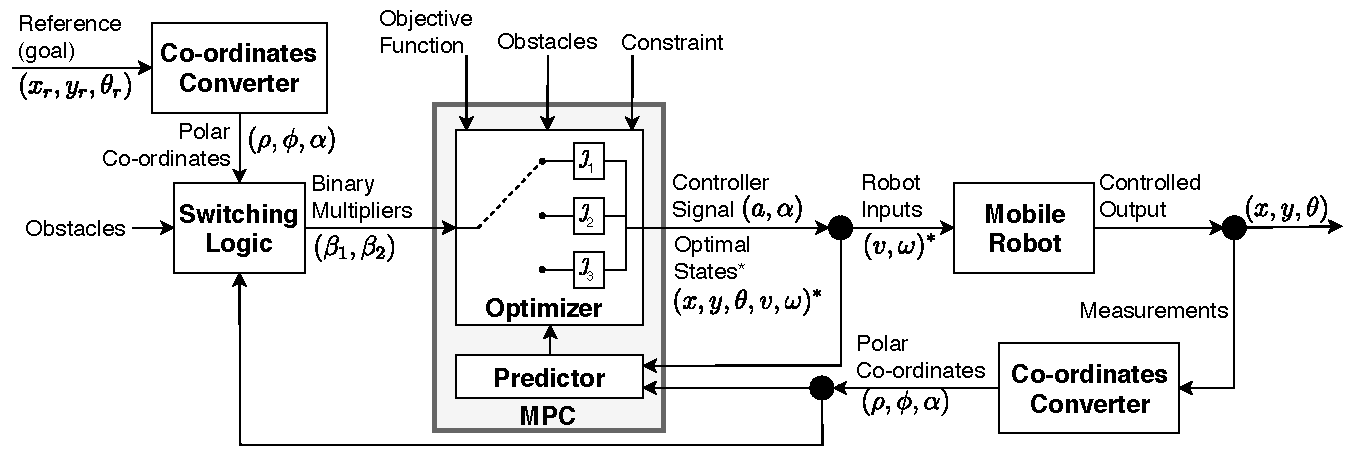
\includegraphics[scale=0.65]{pictures/block_diagram_polar_switch_1.pdf}
			\caption{NMPC Control Loop with Switching Objective}
		\end{figure}
	\end{frame}

	\begin{frame}
		\frametitle{Scenario \textrm{IV}: Dynamic Environment}
		\begin{figure}[hbtp]
			\centering
			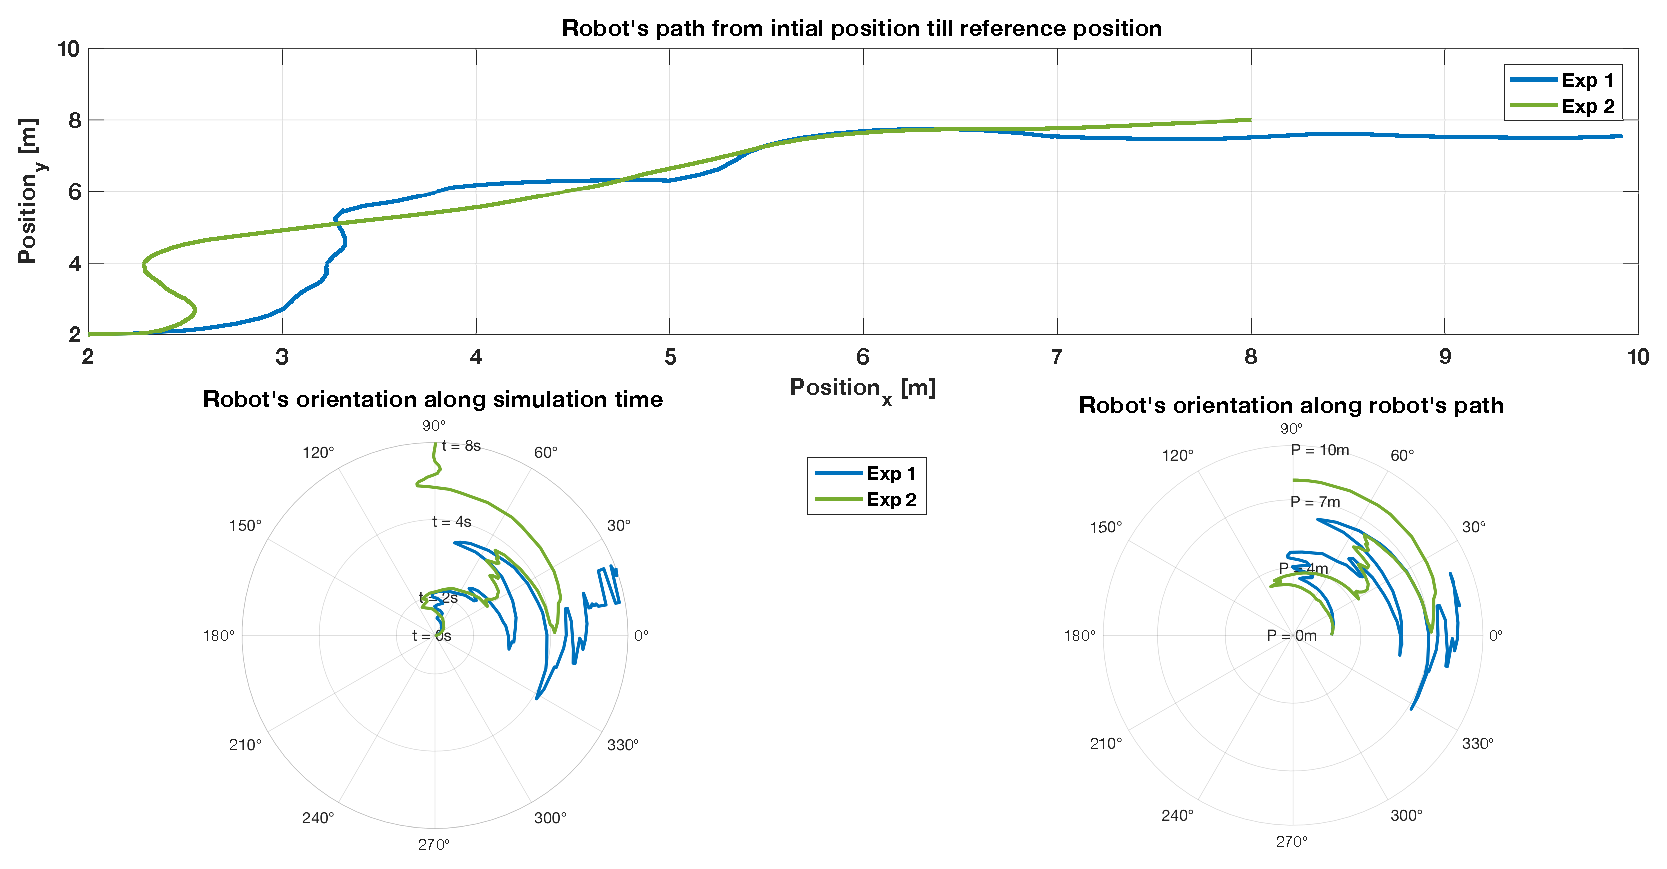
\includegraphics[scale=0.44]{pictures/graphs/sn3_states.eps}
			\caption{State Trajectory Evolution}
		\end{figure}
	\end{frame}
	
	\begin{frame}
		\frametitle{Scenario \textrm{IV}: Dynamic Environment}
		\begin{figure}[hbtp]
			\centering
			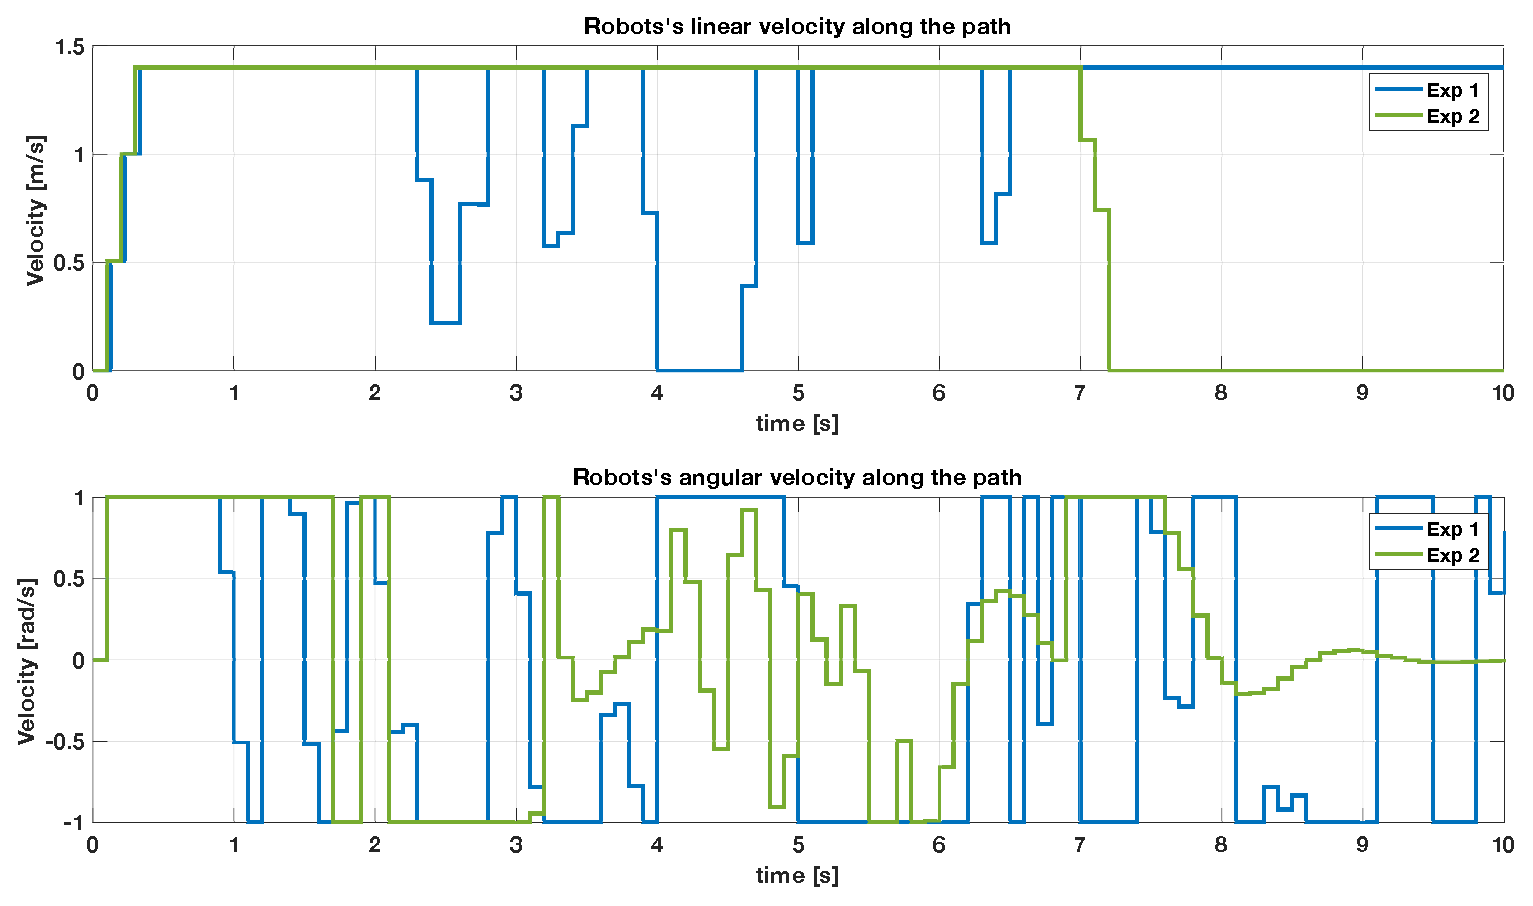
\includegraphics[scale=0.42]{pictures/graphs/sn3_inputs.eps}
			\caption{Input Trajectory Evolution}
		\end{figure}
	\end{frame}
	
	\begin{frame}
		\frametitle{Scenario \textrm{IV}: Dynamic Environment}
		\begin{figure}[hbtp]
			\centering
			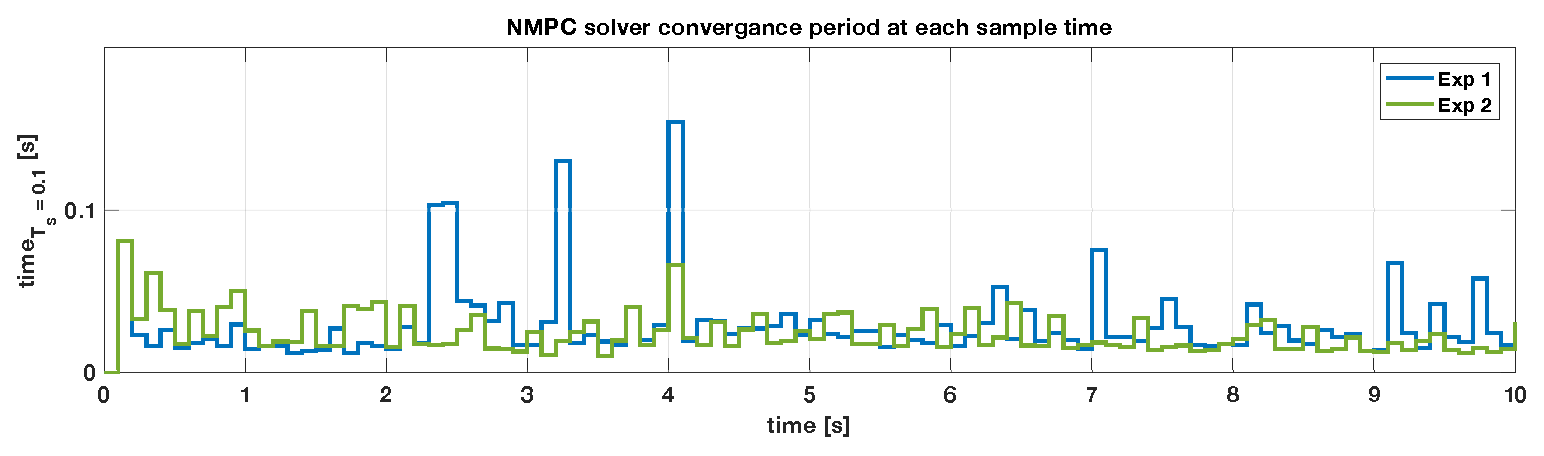
\includegraphics[scale=0.42]{pictures/graphs/sn3_solver_time.eps}
			\caption{NMPC Computational Effort}
		\end{figure}
	\end{frame}
	
	\begin{frame}
		\frametitle{Scenario \textrm{IV}: Dynamic Environment}
		\centering
		\movie[width=0.451\textwidth, height=0.865\textheight]
		{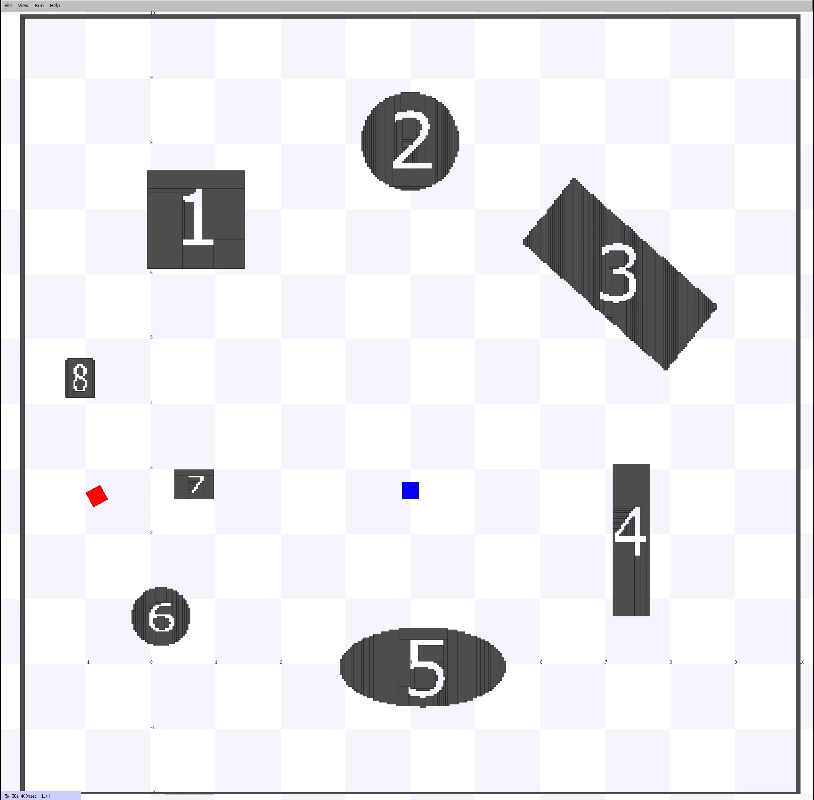
\includegraphics[width=0.45\textwidth]{pictures/good_1.png}}{videos/good_1.mov}
		\nocite{hoy_matveev_savkin_2015}
	\end{frame}

% Datenbanken
% \section{NMPC Planner}

	\begin{frame}
		\centering
		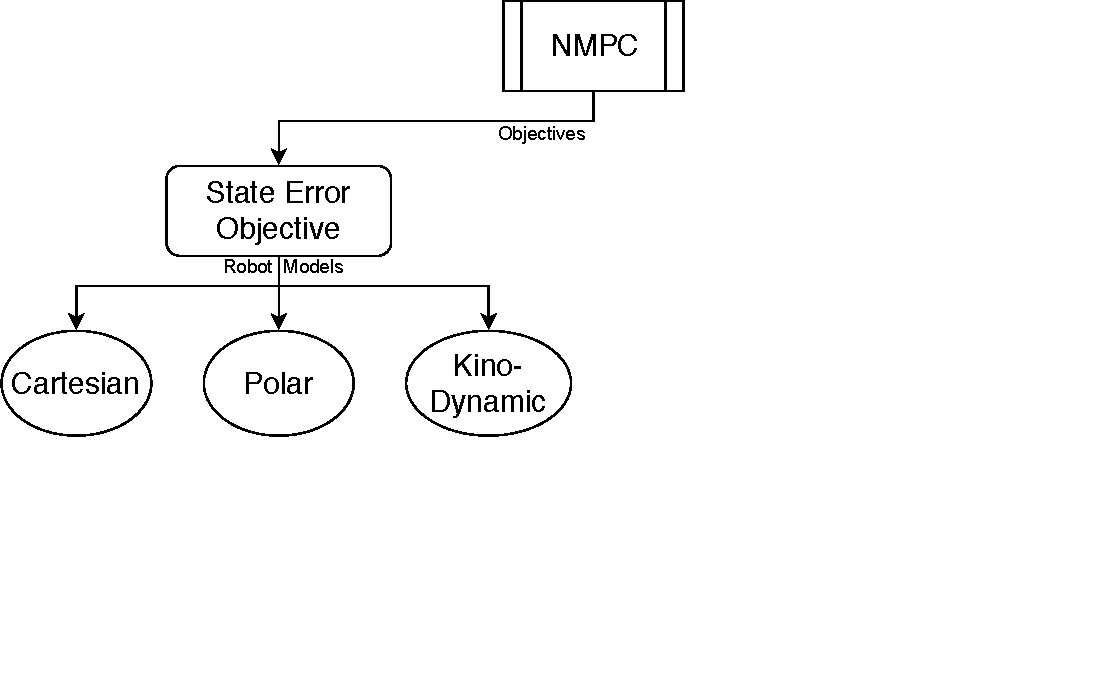
\includegraphics[scale=0.7]{pictures/mpc_planner_group/mpc_planner_8.pdf}
	\end{frame}

	\begin{frame}
		\frametitle{Robot Models Used}
		\begin{columns}[T]
			\begin{column}{0.45\textwidth}
				\onslide<2->{
				\begin{block}{Cartesian Co-ordinate Model}
					\[
					\begin{bmatrix}
						\dot{x} \\
						\dot{y} \\
						\dot{\theta}
					\end{bmatrix}
					=
					\begin{bmatrix}
						\cos(\theta) & 0 \\
						\sin(\theta) & 0 \\
						0 & 1
					\end{bmatrix}
					\begin{bmatrix}
						\upsilon \\
						\omega 
					\end{bmatrix}
					\]
				\end{block}
				}
				\onslide<3->{
				\begin{block}{Kino-dynamic Model}
					\[
					\begin{bmatrix}
						\dot{x} \\
						\dot{y} \\
						\dot{\theta} \\
						\dot{\upsilon} \\
						\dot{\omega}
					\end{bmatrix}
					=
					\begin{bmatrix}
						\cos(\theta) & 0 & 0 & 0 \\
						\sin(\theta) & 0 & 0 & 0 \\
						0 & 1 & 0 & 0 \\
						0 & 0 & 1 & 0 \\
						0 & 0 & 0 & 1
					\end{bmatrix}
					\begin{bmatrix}
						\upsilon \\
						\omega \\
						a \\
						\alpha
					\end{bmatrix}
					\]
				\end{block}
				}
			\end{column}
			\begin{column}{0.49\textwidth}
				\centering
				\onslide<1->{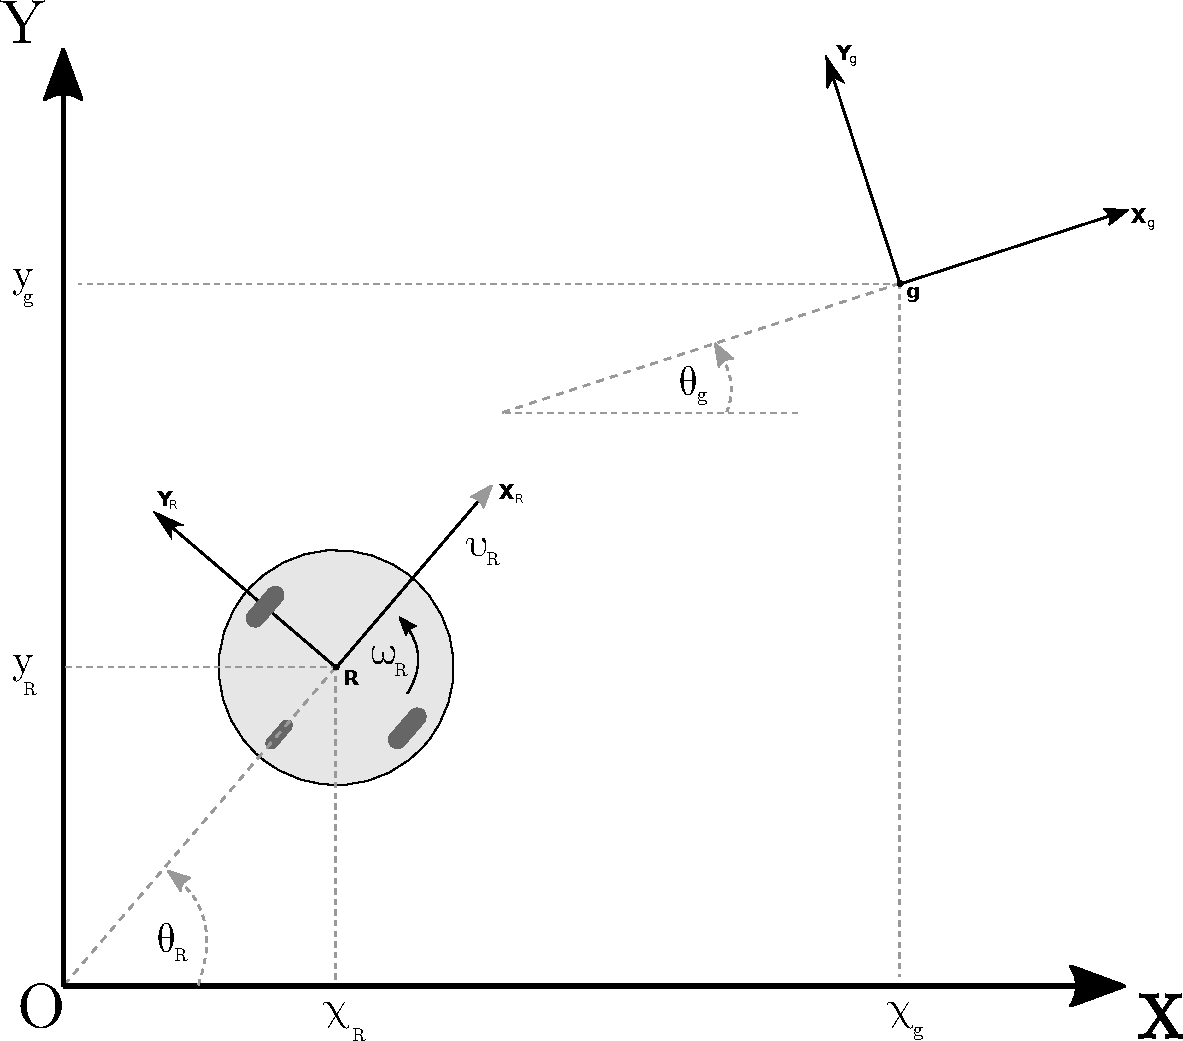
\includegraphics[scale=0.35]{pictures/robot_cart.pdf}}
			\end{column}
		\end{columns}
	\end{frame}

	\begin{frame}
		\frametitle{Robot Models Used}
		\begin{columns}[T]
			\begin{column}{0.45\textwidth}
				\onslide<2->{
				\begin{block}{Polar Co-ordinate Model}
					\begin{align*}
						\rho& = \sqrt{x^2+y^2} \\
						\phi& = \arctan2(y,x) \\
						\alpha&= \phi - \theta
					\end{align*}
				\end{block}
				}
			\end{column}
			\begin{column}{0.49\textwidth}
				\centering
				\onslide<1->{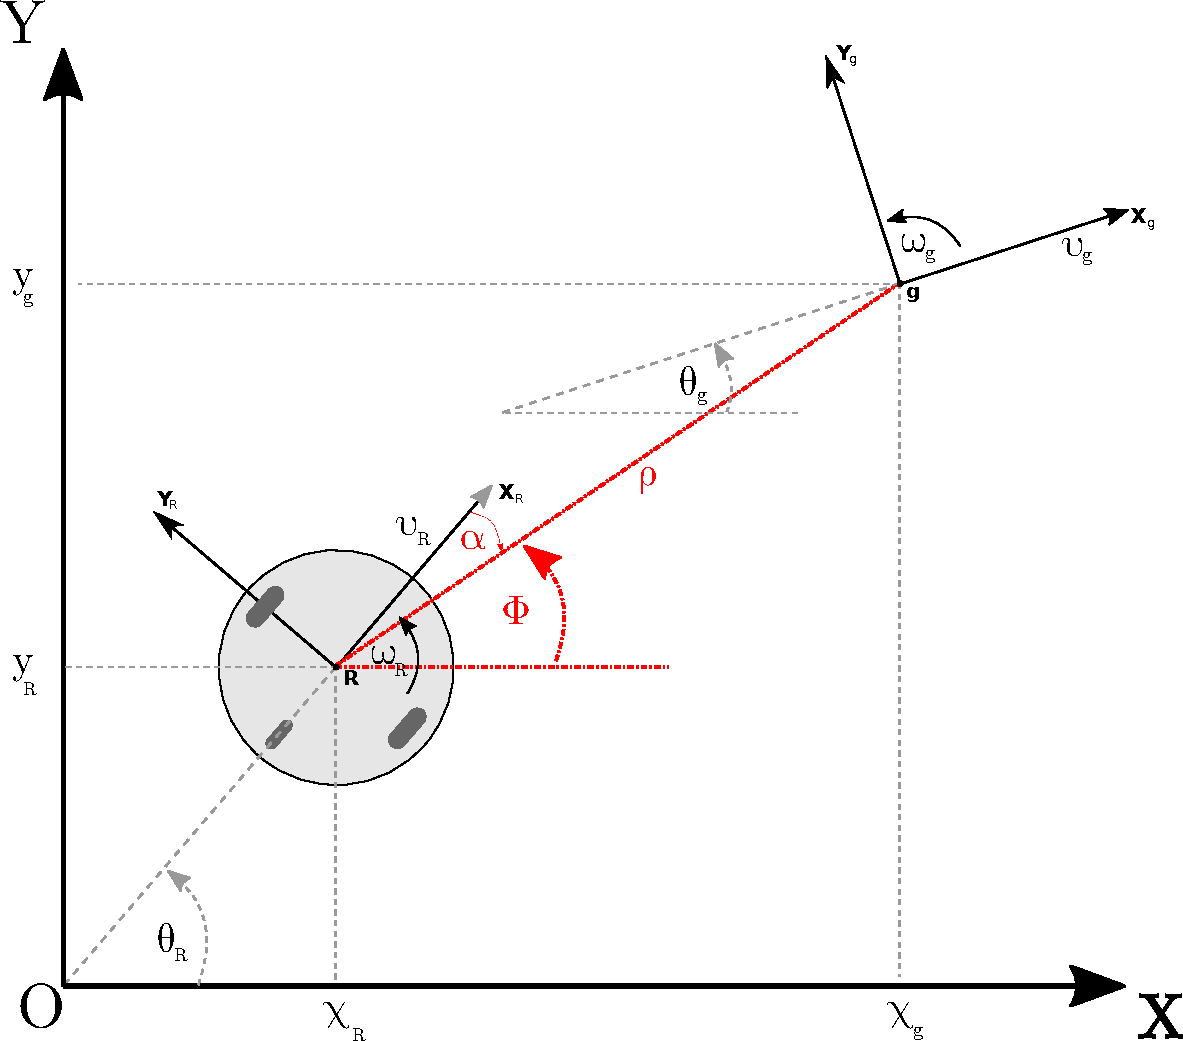
\includegraphics[scale=0.35]{pictures/robot_polar.pdf}}
			\end{column}
		\end{columns}
	\end{frame}

	\begin{frame}
		\frametitle{NMPC General Formulation}
		\begin{block}{NMPC Optimization Problem}
			\begin{align*}
				&\underset{\mathbf{X}^*,\mathbf{U}^*}{\text{min    }}
				\tikzmark{a9}J_{N_p}(\mathbf{x}_k) = \tikzmark{a10}V_f(\mathbf{x}_{k+N_p}) + \sum_{j=0}^{N_p-1}\tikzmark{a11}\ell (\mathbf{x}_{k + j},\mathbf{u}_{k + j}), \\
				&\quad \text{subject to:} \notag  \\
				&\quad\quad \tikzmark{a12}\mathbf{x}_{k+j+1} = \mathcal{F}(\mathbf{x}_{k+j},\mathbf{u}_{k+j}), & \forall\text{ } 0\leq j\leq N_p-1  \\ 
				&\quad\quad \tikzmark{a13}\mathbf{x}_{k+j} \in \mathbb{X}, & \forall \text{ }0\leq j\leq N_p \\
				&\quad\quad \tikzmark{a14}\mathbf{u}_{k+j} \in \mathbb{U}, & \forall \text{ }0\leq j\leq N_p-1 \\
				&\quad\quad \tikzmark{a15}\mathbf{d}_{\imath,k+j}  \geq \xi_o, & \forall\text{ } 0\leq j\leq N_p-1, \text{ }\forall\text{ } \imath \in I_s
			\end{align*}
		\end{block}
	
		\begin{tikzpicture}[overlay, remember picture]
			\coordinate (A9) at ($({pic cs:a9})+(1ex, 1ex)$);
			\coordinate (A10) at ($({pic cs:a10})+(1ex, 1ex)$);
			\coordinate (A11) at ($({pic cs:a11})+(1ex, 1ex)$);
			\coordinate (A12) at ($({pic cs:a12})+(0ex, 0.5ex)$);
			\coordinate (A13) at ($({pic cs:a13})+(0ex, 0.5ex)$);
			\coordinate (A14) at ($({pic cs:a14})+(0ex, 0.5ex)$);
			\coordinate (A15) at ($({pic cs:a15})+(1ex, -0.5ex)$);
			\pause
			\node [fit=(A9), baseline] (n9) {};
			\node[cyan, above of= n9, node distance = 3em] (t9_1) {\small cost};
			\node[cyan, above of= n9, node distance = 2em] (t9) {\small function};
			\draw [<-, cyan] (n9.north) to [below] (t9.south);
			\pause
			\node [fit=(A10), baseline] (n10) {};
			\node[cyan, above of= n10, node distance = 3em] (t10_1) {\small terminal};
			\node[cyan, above of= n10, node distance = 2em] (t10) {\small penalty};
			\draw [<-, cyan] (n10.north) to [below] (t10.south);
			\pause
			\node [fit=(A11), baseline] (n11) {};
			\node[cyan, above of= n11, node distance = 3em] (t11_1) {\small regulatory};
			\node[cyan, above of= n11, node distance = 2em] (t11) {\small term};
			\draw [<-, cyan] (n11.north) to [below] (t11.south);
			\pause
			\node [fit=(A12), baseline] (n12) {};
			\node[cyan, left of= n12, node distance = 4em] at (2,3) (t12) {\small model};
			\node[cyan, below of= t12, node distance = 1em] (t12_1) {\small constraints};
			\draw [<-, cyan] (n12.west) to [right] (t12.east);
			\pause
			\node [fit=(A13), baseline] (n13) {};
			\node[cyan, left of= n13, node distance = 4em] (t13) {\small state};
			\node[cyan, below of= t13, node distance = 1em] (t13_1) {\small boundries};
			\draw [<-, cyan] (n13.west) to [right] (t13.east);
			\pause
			\node [fit=(A14), baseline] (n14) {};
			\node[cyan, left of= n14, node distance = 4em] at (2,1) (t14) {\small input};
			\node[cyan, below of= t14, node distance = 1em] (t14_1) {\small boundries};
			\draw [<-, cyan] (n14.west) to [right] (t14.east);
			\pause
			\node [fit=(A15), baseline] (n15) {};
			\node[cyan, below of= n15, node distance = 3em] (t15_1) {\small static};
			\node[cyan, below of= n15, node distance = 2em] (t15) {\small obstacles};
			\draw [<-, cyan] (n15.south) to [above] (t15.north);
		\end{tikzpicture}
	\end{frame}
	
	\begin{frame}
		\frametitle{NMPC General Formulation}
		\begin{block}{Regulatory Terms (e.g., Cartesian coordinate)}
			\[
				\begin{aligned}
					\ell (\mathbf{x}_{k + j},\mathbf{u}_{k + j}) = \enspace
					\tikzmark{a1}
					(\mathbf{x}_{k + j} - \mathbf{x}_{ref})^T \enspace Q_1 \enspace (\mathbf{x}_{k + j} - \mathbf{x}_{ref})
					\tikzmark{a2}
					\enspace + \enspace
					\tikzmark{a3}
					\Delta\mathbf{u}_{k + j}^T \enspace R \enspace \Delta\mathbf{u}_{k + j}
					\tikzmark{a4}
					\enspace \tikzmark{a7}-\tikzmark{a8} \enspace
					\tikzmark{a5} 
					\sum_{i=0}^{I} \mathbf{d}_{i,k + j}^T \enspace Q_2 \enspace \mathbf{d}_{i,k + j}
					\tikzmark{a6}
				\end{aligned}
			\]
		\end{block}
		\vfill
		\vfill
		\vfill
		\begin{itemize}
			\item $\mathbf{d}_{i,k + j}$: distance between the robot and $i^{th}$ detected moving obstacle.
		\end{itemize}
		
		\begin{tikzpicture}[overlay, remember picture]
			\coordinate (A1) at ($({pic cs:a1})+(+0.1ex, 2ex)$);
			\coordinate (A2) at ($({pic cs:a2})+(-0.1ex,-0.5ex)$);
			\coordinate (A3) at ($({pic cs:a3})+(+0.1ex, 2ex)$);
			\coordinate (A4) at ($({pic cs:a4})+(-0.1ex,-0.5ex)$);
			\coordinate (A5) at ($({pic cs:a5})+(+0.1ex, 3.5ex)$);
			\coordinate (A6) at ($({pic cs:a6})+(-0.1ex,-2.5ex)$);
			\coordinate (A7) at ($({pic cs:a7})+(+1ex, 0.5ex)$);
			\coordinate (A8) at ($({pic cs:a8})+(-1ex, 0.5ex)$);
			\pause
			\node [fit=(A1)(A2), draw=tugreen, thick, rounded corners] (n1) {};
			\node[overlay, below of= n1, node distance = 6em] (t1) {State Error};
			\node[overlay, below of= n1, node distance = 7em] (t1_1) {Objective};
			\draw [thick, -latex, tugreen] (n1.south) to [above] (t1.north);
			\pause
			\node [fit=(A3)(A4), draw=tugreen, thick, rounded corners] (n2) {};
			\node[overlay, below of= n2, node distance = 6em] (t2) {Input Penealty};
			\node[overlay, below of= n2, node distance = 7em] (t2_1) {Objective};
			\draw [thick, -latex, tugreen] (n2.south) to [above] (t2.north);
			\pause
			\node [fit=(A5)(A6), draw=tugreen, thick, rounded corners] (n3) {};
			\node[overlay, below of= n3, node distance = 5.7em] (t3) {Dyn Obstacles};
			\node[overlay, below of= n3, node distance = 6.7em] (t3_1) {Objective};
			\draw [thick, -latex, tugreen] (n3.south) to [above] (t3.north);
			\pause
			\node [fit=(A7)(A8), draw=red, circle] (n4) {};
			\node[overlay, red, above of= n4, node distance = 8em] (t4) {Maximization};
			\draw [thick, -latex, red] (n4.north) to [below] (t4.south);
		\end{tikzpicture}
		
%		\tikz[baseline=(n1.base)]{
%			\node[draw=tugreen, ,thick, rounded corners, inner sep=5pt] 
%			(n1){$xfoz$};
%			\node[overlay, below of= n1, node distance = 6em] (t1) {State Error};
%			\draw [thick, -latex, tugreen] (n1.south) to [above] (t1.north);
%		}
	\end{frame}
	
	\begin{frame}
		\frametitle{Potential Collision Zone}
		\centering
		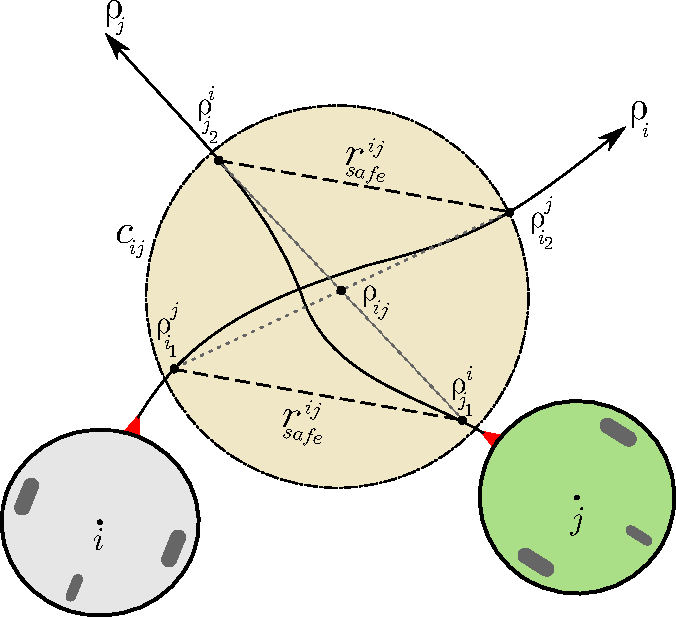
\includegraphics[scale=0.6]{pictures/robots_pot_coll.pdf}
	\end{frame}
	
	\begin{frame}
		\frametitle{Cartesian Coordinate Model Block Diagram}
		\begin{figure}[hbtp]
			\centering
			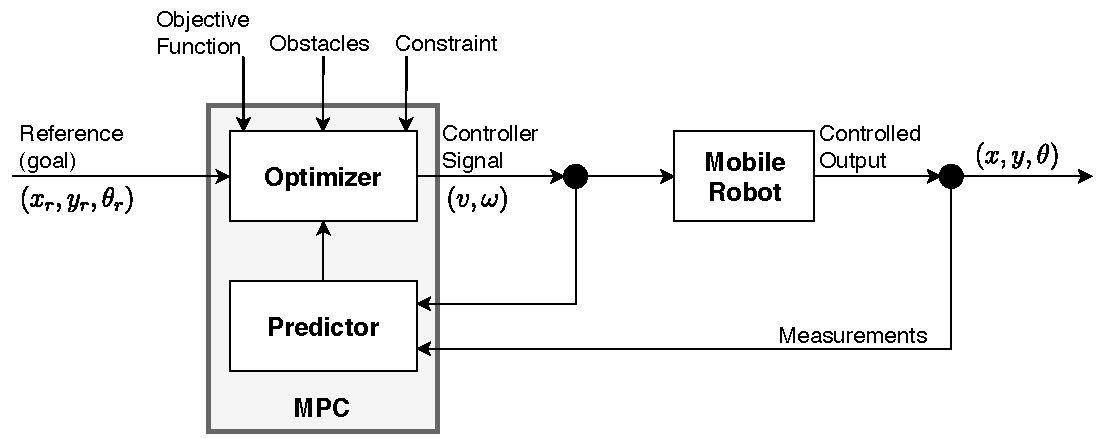
\includegraphics[scale=0.7]{pictures/block_diagram_cart.pdf}
			\caption{NMPC Control Loop (Cartesian coordinate Model)}
		\end{figure}
	\end{frame}

	\begin{frame}
		\frametitle{Polar Coordinate Model}
		\begin{block}{Regulatory Term}
			\parbox[c][4\baselineskip][t]{\textwidth}{
			\begin{align*}
				\ell_p (\vartheta_{k + j},\mathbf{u}_{k + j}) &= 
				\pmb{[} \ell_{p,1}(\cdot,\cdot) \enspace \ell_{p,2}(\cdot,\cdot) \enspace \ell_{p,3}(\cdot,\cdot) \pmb{]}
				\enspace
				\mathbf{Q_1} \enspace
				\begin{bmatrix}
					\ell_{p,1}(\cdot,\cdot) \\
					\ell_{p,2}(\cdot,\cdot) \\
					\ell_{p,3}(\cdot,\cdot)
				\end{bmatrix}
				+ \cdots
			\end{align*}
			}
		\end{block}
		Minimization of:
		\begin{itemize}
			\item Euclidean distance: $\ell_{p,1}(\cdot,\cdot) = \sqrt{(x_{k+j} - x_{ref})^2+(y_{k+j} - y_{ref})^2}$
			\item Heading towards goal: $\ell_{p,2}(\cdot,\cdot) = \Big(\theta_{k+j} - \arctan2\big((y_{k+j} - y_{ref}),(x_{k+j} - x_{ref})\big)\Big)^2$
			\item Reference orientation: $\ell_{p,3}(\cdot,\cdot) = (\theta_{k+j} - \theta_{ref})^2$
		\end{itemize}
	\end{frame}

	\begin{frame}
		\frametitle{Polar Coordinate Model Block Diagram}
		\begin{figure}[hbtp]
			\centering
			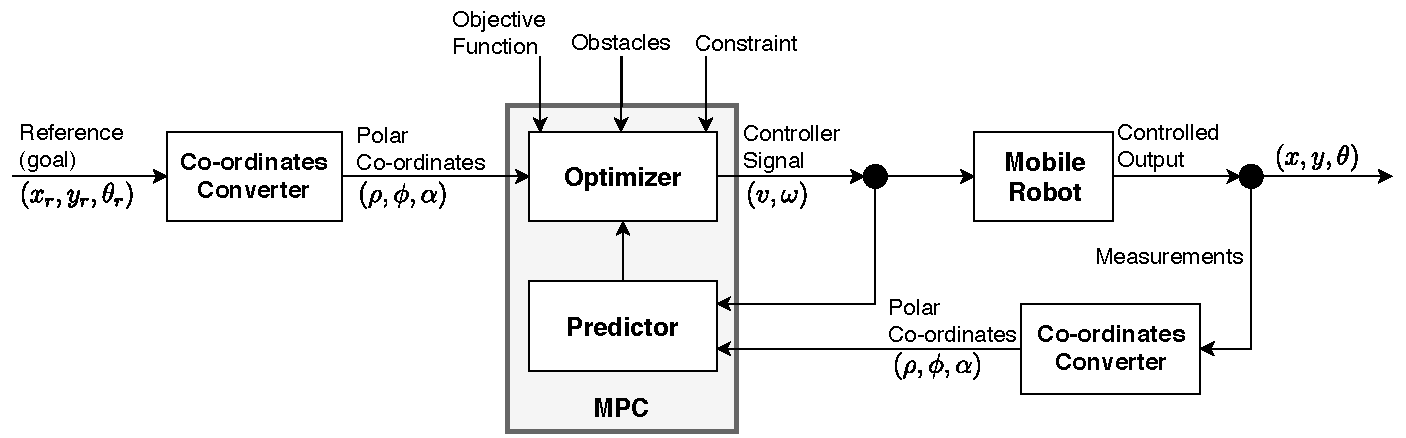
\includegraphics[scale=0.64]{pictures/block_diagram_polar.pdf}
			\caption{NMPC Control Loop (Polar coordinate Model)}
		\end{figure}
	\end{frame}

	\begin{frame}
		\frametitle{Kino-dynamic Model Block Diagram}
		\begin{figure}[hbtp]
			\centering
			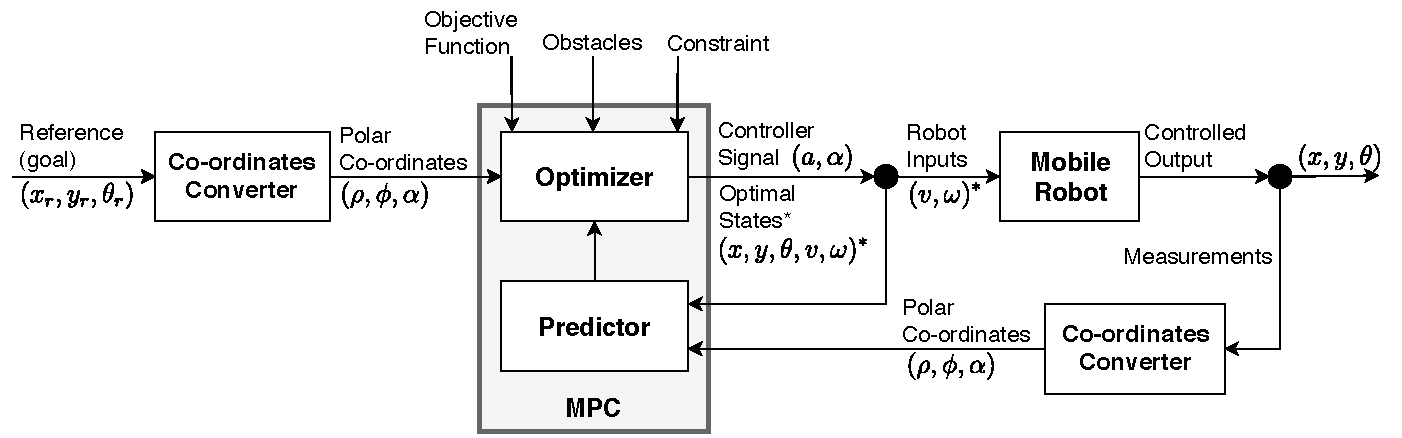
\includegraphics[scale=0.64]{pictures/block_diagram_kino.pdf}
			\caption{NMPC Control Loop (Kino-dynamic Model)}
		\end{figure}
	\end{frame}



%Quellenverzeichnis
\begin{frame}[allowframebreaks]
        \frametitle{Quellenverzeichnis}
        %\bibliographystyle{plain}
        \printbibliography
\end{frame}
\end{document}
